\documentclass[11pt,a4paper]{article}
\usepackage[margin=0.85in]{geometry}
\usepackage{amsmath,amssymb}
\usepackage{newtxtext,newtxmath}
\usepackage{microtype}
\usepackage{enumitem,framed}
\usepackage{booktabs,longtable,array,tabularx}
\usepackage[numbers,sort&compress]{natbib}
\usepackage{tikz}
\usetikzlibrary{arrows.meta,positioning,calc,fit,backgrounds,shapes.geometric}
\tikzset{every node/.style={execute at begin node={\hyphenpenalty=10000\exhyphenpenalty=10000}}}
\usepackage{caption}
\captionsetup{font=small,labelfont=bf,skip=6pt}
\usepackage[section]{placeins}
\usepackage{xcolor}
\definecolor{linkblue}{HTML}{174D75}
\definecolor{humanred}{HTML}{A23B2A}
\definecolor{planegray}{HTML}{5A6270}
\definecolor{reviewgreen}{HTML}{2E6B3A}
\definecolor{standorange}{HTML}{B56A14}
\definecolor{methodpurple}{HTML}{5E3A87}
\usepackage[colorlinks=true,linkcolor=linkblue,citecolor=linkblue,urlcolor=linkblue,breaklinks=true]{hyperref}
\hypersetup{pdftitle={Human-in-the-Loop Automated Research: Verification-Centered Scientific Discovery},
 pdfsubject={Human scientific direction, anti-inflation formalization, executable review, and scholarly validation},
 pdfkeywords={human-in-the-loop automated research, scientific discovery, scientific slop, formal verification, Lean 4, executable peer review, scholarly collaboration}}
\urlstyle{same}
\setlength{\emergencystretch}{2.5em}
\setlength{\parskip}{3pt}
\setlength{\parindent}{1.2em}
\setlength{\tabcolsep}{4pt}
\setlength{\textfloatsep}{12pt plus 2pt minus 2pt}
\raggedbottom
\renewcommand{\topfraction}{0.95}
\renewcommand{\bottomfraction}{0.95}
\renewcommand{\textfraction}{0.05}
\renewcommand{\floatpagefraction}{0.85}
\setcounter{topnumber}{4}
\setcounter{totalnumber}{5}
\makeatletter
\setlength{\@fptop}{0pt}
\setlength{\@fpsep}{12pt}
\setlength{\@fpbot}{0pt plus 1fil}
\makeatother
\setlist{leftmargin=*,itemsep=2pt,topsep=4pt}
\newcommand{\arxiv}[1]{\href{https://arxiv.org/abs/#1}{\texttt{#1}}}
\newcommand{\code}[1]{\texttt{\detokenize{#1}}}
\newcommand{\gh}[2]{\href{https://github.com/#1}{#2}}
\newcolumntype{L}[1]{>{\raggedright\arraybackslash}p{#1}}
\newcolumntype{Y}{>{\raggedright\arraybackslash}X}
\newcounter{protocolbox}
\newenvironment{protocol}[1]{\refstepcounter{protocolbox}\begin{framed}\noindent\textbf{Box~\theprotocolbox.\ #1}\par\small}{\end{framed}}
\newcommand{\authorblock}{%
Chloe Chew$^{1}$, Abigail Deng$^{1}$, Zongzhe Huang$^{1}$, Louis Li$^{1}$, Rona Liang$^{1}$,
Kai Huei Lim$^{1}$, Kai Wei Lim$^{1}$, Yitian Liu$^{1}$, Haobo Ma$^{1}$, Wen Niu$^{1}$,
Jianwei Su$^{1}$, Calvin Tan$^{1}$, Haylee Wang$^{1}$, Jason Wang$^{1}$,
Shining Wang$^{1}$, Wenlin Zhang$^{1,2}$\\[4pt]
{\small $^{1}$ChronoAI Pte Ltd, Singapore \quad $^{2}$National University of Singapore, Singapore}\\[3pt]
{\footnotesize Authors are listed in alphabetical order by surname.}}

\begin{document}
\begin{titlepage}
\begin{center}
{\LARGE Human-in-the-Loop Automated Research:\\[3pt]
Verification-Centered Scientific Discovery\par}
\vspace{0.6em}
{\large Human scientific direction, anti-inflation formalization,\\
executable review, and scholarly validation\par}
\vspace{0.9em}
{\normalsize\authorblock\par}
\vspace{0.6em}
Working manuscript, 27 November 2026
\end{center}
\vspace{0.5em}
\begin{abstract}
Scientific discovery is defined by the ability to recognize the boundaries of
existing knowledge, decide which questions matter, and establish new truths
that a scholarly community can inspect and build upon. As foundation models and
neural theorem provers shift theoretical research from proof scarcity toward
automated abundance, artificial intelligence is moving from a passive assistant
to an active partner in discovery. Yet full autonomy without human guidance or
formal grounding faces a sharp failure mode: unguided agents generate locally
plausible ``scientific slop'' whose global logic collapses, while unchecked
theorem provers produce opaque formal code (``proof indigestion'') that
outpaces human comprehension. Here we introduce a verification-centered,
human-in-the-loop methodology for automated scientific discovery and evaluate
it on its strictest deductive proving ground across mathematics, quantum
information, mathematical physics and theoretical computer science.
Specifically, human researchers provide scientific direction (from sharp open
conjectures to embryonic conceptual intuitions), redirect false premises and
evaluate the readable proof. An open, model-agnostic orchestration harness
stores authoritative state outside any single model and coordinates derivation,
counterexample search, cold cross-family adversarial critique and four
anti-inflation Lean~4 admission gates. Internal review translates disputed
claims into executable verification targets, while direct collaboration with
living domain scholars reconnects machine-checked arguments to human
understanding. Across 30 public manuscripts evaluated blindly by three
independent frontier model families (OpenAI Codex, Anthropic Claude and Google
Gemini; 90 evaluations; Kendall concordance $W=0.828$), collaborative preprints
rank highest under every judge, outperforming autonomous AI-only studies in 260
of 300 cross-cohort comparisons (exact permutation $p=0.0012$, $0.0149$ and
$3.2\times10^{-5}$), matching sound human-only arXiv preprints with 2.3- to
4.2-fold narrower overall dispersion and carrying formal or certified checks in
all ten papers versus one of ten human preprints and none of ten autonomous
studies. A controlled ablation over 20 real mathematical claims shows that
enforcing an executable counterexample witness eliminates false-positive
``review slop'' while retaining high flaw recall, and an audit of 24,925 public
formal-gate contributions documents systematic pre-admission rejection and
multi-commit repair. Together with 17 collaborative arXiv preprints (16 with
external coauthors), 177 proof-checking scholars and an instrumented 33-hour
research trace, these results show how human-guided, verification-centered
automation can expand the frontier of rigorous scientific knowledge.
\end{abstract}
\vspace{0.5em}
\noindent\textbf{Keywords:} human-in-the-loop automated research; scientific
discovery; scientific slop; Lean~4; formal verification; executable peer
review; scholarly collaboration.
\end{titlepage}
\setcounter{page}{2}

\section{Introduction}
Scientific discovery has long been defined by the capacity to locate the
boundaries of existing knowledge and establish new truths that endure under
scrutiny. With rapid advances in foundation models and neural theorem provers,
artificial intelligence is transitioning from a passive conversational
assistant into an active participant in the research process
\citep{tao2026age,scientisttwo}. This shift is moving theoretical disciplines
from proof scarcity toward automated abundance. Yet expanding the scientific
frontier requires far more than generating fluent manuscripts or formal code at
speed. Without sustained human involvement and non-circular verification,
automated research breaks down from two opposite directions. On the informal
side, autonomous paper generators produce ``scientific slop'': manuscripts
whose local paragraphs and equations read smoothly while global logic,
attribution and evidentiary grounding collapse \citep{oh2026slop,societyai}. On
the formal side, Terence Tao in his 2026 International Congress of
Mathematicians lecture and the signatories of the Leiden Declaration warn that
releasing opaque machine proofs without readable exposition or scholarly
dialogue creates ``proof indigestion'', weakening human comprehension and
eroding the living communities that sustain a discipline
\citep{tao2026age,leiden2026}.

Existing automated research architectures leave four fundamental requirements
unresolved. In \emph{A Society of AI Scientists}, 936 autonomous agents across
35 laboratories produced 936 studies, yet blinded evaluation over 202 matched
pairs rated them below human preprints in novelty (7.05 versus 7.45) and
significance (7.04 versus 7.34), with overclaiming in 73\% of first-day
manuscripts and text-only AI referees flagging 10 of 16 repaired drafts versus
11 of 16 broken originals \citep{societyai}. Literature-grounded automated
reviewers such as Stanford Agentic Reviewer and OpenAIReview improve prose
critique, yet their outputs remain unverified text: the strongest OpenAIReview
configuration missed 28.4\% of injected errors across eight arXiv fields
\citep{stanford,nguyen2026review}, and recent peer-review analysis in
\emph{Nature Machine Intelligence} warns that low-cost AI criticism overwhelms
authors with false-positive ``review slop'' unless objections clear an explicit
``obligation threshold'' \citep{sun2026obligation}. Meanwhile, standalone
theorem provers certify logical validity for a given syntax without curating
significance or curbing synthetic library inflation, and session-bound coding
agents lose verified state whenever models or tasks change.

To overcome these challenges, we introduce a verification-centered,
human-in-the-loop methodology for automated scientific discovery and evaluate
it on its strictest deductive proving ground across mathematics, quantum
information, mathematical physics and theoretical computer science. Our
framework rests on a clear division of labor: human researchers provide the
scientific vision (from precise open conjectures to embryonic conceptual
intuitions), redirect false premises, evaluate the readable proof and retain
authorship and publication authority, while an open, model-agnostic
orchestration harness executes large-scale derivation, refutation and formal
verification. Four tightly coupled mechanisms anchor the workflow:
\begin{itemize}
\item \textbf{External shared state and model-agnostic orchestration.}
Authoritative objectives, versioned snapshots, claim statuses and gate outcomes
live outside any individual model's conversation window, allowing heterogeneous
reasoning agents, theorem provers and human collaborators to hand off work and
audit every step without vendor lock-in.
\item \textbf{Anti-inflation formal admission.} Every new Lean~4 unit must
clear four public gates (preregistration before probing, library-first reuse,
rejection of bind-only wrappers and an explicit non-trivial escape witness or
verbatim open-problem settlement) before entering the frozen knowledge base.
\item \textbf{Cross-family adversarial critique with executable review
obligations.} Cold reviewers from independent model families attack frozen
snapshots, and disputed claims are converted into executable verification
targets whose deterministic verdict returns directly to the manuscript,
enforcing Sun et al.'s obligation threshold in practice.
\item \textbf{Readable exposition and collaboration with living scholars.}
Bilingual living books pair every frozen formal declaration with self-contained
human prose, and direct collaboration with living domain experts (often the
authors of the original open problems) tests mathematical meaning, attribution
and the next research direction.
\end{itemize}

We evaluate this methodology through five converging lines of empirical
evidence. First, in a blinded external benchmark of 30 public manuscripts
scored independently by three named frontier model families (OpenAI Codex
\code{gpt-6.1-sol}, Anthropic Claude \code{claude-opus-5-5} and Google Gemini;
90 evaluations; Kendall concordance $W=0.828$), collaborative preprints rank
highest under every judge, outperforming autonomous AI-only studies in 260 of
300 cross-cohort comparisons (exact permutation $p=0.0012$, $0.0149$ and
$3.2\times10^{-5}$), matching sound human-only arXiv preprints with 2.3- to
4.2-fold narrower overall dispersion and carrying formal or certified checks in
all ten papers versus one of ten human preprints and none of ten autonomous
studies. Second, version-blinded longitudinal arXiv revisions tie large score
gains directly to mathematical repairs, including a 4.2-point jump over 30
days. Third, a controlled 20-claim mechanistic ablation across real
mathematical theorems and counterexamples from this corpus demonstrates how an
executable counterexample gate eliminates false-positive prose review slop
while maintaining high flaw recall. Fourth, a public audit of 24,925 completed
Lean~4 gate submissions documents systematic pre-admission rejection and
multi-commit repair. Fifth, across the live programme, 17 collaborative arXiv
preprints (16 with external academic coauthors), 177 proof-checking living
scholars and an instrumented 33-hour research trace (31 brief human directives
guiding six kernel-verified Lean~4 units and 52 early refutations) show human
digestion working in practice. Sections~\ref{sec:position}
and~\ref{sec:methods} diagnose why unguided automation stalls and specify our
architecture; Sections~\ref{sec:results} and~\ref{sec:discussion} present the
empirical evaluation, design principles, future outlook and limitations, with
programme counts and archived reproducibility records in
Appendix~\ref{app:repro}.

\section{Why Unguided Automation Stalls}
\label{sec:position}
Automated scientific discovery has advanced along three largely separate
tracks: autonomous paper generation, formal theorem proving and automated peer
review, building on earlier robot-scientist and AI-for-science frameworks
\citep{king,gil,kitano,wangsci,deepresearchsurvey}. Taken in isolation, none of
these tracks prevents the twin failures emerging at scale: scientific slop on
the informal side and proof indigestion on the formal side. Examining where
current architectures break across the research stack defines the exact
requirements for human-in-the-loop verification.

\paragraph{Scientific slop and proof indigestion.}
As automated tools shift theoretical work from proof scarcity to proof
abundance, Terence Tao distinguishes five stages in a healthy research pipeline
(solving, verification, exposition, peer review and community digestion). He
warns that accelerating only the first two stages produces ``proof
indigestion'' whenever opaque machine outputs outpace human understanding and
fail the ``chalkboard test'' of genuine mastery \citep{tao2026age}. The Leiden
Declaration echoes this warning across the mathematical community, highlighting
plausible yet flawed AI arguments, weakened attribution and eroding human
agency over research agendas \citep{leiden2026}. Empirical audits confirm the
prose pathology. In \emph{Science or Slop?}, Oh et al.\ benchmark 390
AI-generated papers against matched human manuscripts and show that even when
individual paragraphs read smoothly, global failures in structure, argument
coherence and evidentiary grounding identify AI-generated slop with 85.9\%
accuracy and track human peer-review rejections \citep{oh2026slop}. Likewise,
the 936 autonomous studies in \emph{A Society of AI Scientists} trail human
preprints in novelty and significance, show 73\% first-day overclaiming and
confuse text-only AI referees on broken versus repaired drafts
\citep{societyai}. Scaling autonomous generation without human direction at
entry and readable verification at exit increases manuscript volume faster than
scientific insight.

\paragraph{Paper generators and coding agents without persistent formal grounding.}
A growing body of autonomous systems links idea generation, code execution and
manuscript drafting into end-to-end loops, including The AI Scientist and AI
Scientist-v2 \citep{aiscientist,scientistv2}, DeepScientist
\citep{deepscientist}, AI-Researcher \citep{airesearcher}, Kosmos
\citep{kosmos}, PaperOrchestra \citep{paperorchestra}, CycleResearcher
\citep{cycleresearcher}, and Google's ScientistOne and ScientistTwo, which tie
experimental evidence chains to screening, ablations and review and rebuttal
cycles \citep{scientistone,scientisttwo}. Human-guided systems keep scientists
inside experimental loops: Agent Laboratory, CodeScientist and
AutoResearchClaw retain iterative human oversight over code-based exploration
\citep{agentlab,codescientist,autoresearchclaw}, while Co-Scientist and
chemistry agents connect researcher-guided hypotheses to wet-laboratory
experiments \citep{coscientist,boiko2023coscientist,chemcrow}. In algorithmic
and empirical domains, program-search and coding-agent frameworks such as
FunSearch, AlphaEvolve, AIDE, MARS, AutoSOTA, EvoScientist, MLAgentBench and
OpenAI4S optimize against executable benchmarks
\citep{funsearch,alphaevolve,aide,mars,autosota,evoscientist,mlagentbench,openai4s},
building on general agent interfaces and memory layers such as ReAct, AutoGen,
MetaGPT, SWE-agent, OpenHands, Voyager, Reflexion and MemGPT
\citep{react,autogen,metagpt,sweagent,openhands,voyager,reflexion,memgpt}. For
deductive science, empirical heuristics and ephemeral coding sessions leave a
core gap: central claims require machine-checked validity and persistent state
that survives across models, runtimes and multi-week collaborations.

\paragraph{Formal provers without curation, exposition or scholarly closure.}
Formal proof assistants establish deductive ground truth. Lean~4 and its
community library Mathlib \citep{lean4,mathlib} anchor a rapidly advancing
ecosystem of neural theorem provers and interactive tools, ranging from Draft,
Sketch, and Prove, LeanDojo, Lean Copilot and LeanAgent
\citep{dsp,leandojo,leancopilot,leanagent} to DeepSeek-Prover-V1.5 and V2,
Goedel-Prover, Kimina-Prover, Seed-Prover, AlphaProof, Aristotle,
AlphaGeometry and AlphaGeometry2
\citep{deepseekprover15,deepseekprover2,goedel,kimina,seedprover,alphaproof,aristotle,alphageometry,alphageometry2}.
A proof kernel certifies logical entailment, not mathematical value. Left
unguarded, automated provers generate ``formal slop'': hundreds of trivial
specializations and wrappers that bloat shared libraries without advancing a
theorem. Collaborative human-led precedents, including AI-guided mathematical
intuition \citep{davies,georgiev}, Polymath \citep{polymath} and the Equational
Theories Project \citep{etp}, show that lasting progress pairs computational
scale with human problem framing, transparent exposition and peer dialogue.
Drawing on supervisory control and mixed-initiative interaction
\citep{sheridan,parasuraman,horvitz,amershi}, preregistration \citep{nosek},
provenance standards \citep{prov,fair} and auditable agent records
\citep{symposium,verifiedlab,openai4s}, a durable research loop binds formal
validity to explicit human authority and versioned public state.

\paragraph{Automated peer review and obligation thresholds.}
Automated reviewing has progressed rapidly while exposing a sharp structural
asymmetry. Stanford Agentic Reviewer (Jiang and Ng; \code{paperreview.ai})
retrieves arXiv literature to generate prose critiques whose Spearman
correlation with human ICLR~2025 scores reaches 0.42, compared with 0.41 for
agreement between human reviewers \citep{stanford}. When Google's ScientistTwo
uses it as a held-out referee, ScientistTwo manuscripts score $5.7\pm0.6$ (with
72.1\% passing the automated acceptance threshold, versus 7.5 and 91.9\% on the
in-distribution ScholarPeer referee \citep{scientisttwo,scholarpeer}), while
AI-Researcher, CycleResearcher, AI Scientist-v2 and ScientistOne score 0\% at
that held-out threshold. Prose-only reviewing still misses major errors.
Benchmarking OpenAIReview, coarse, Reviewer3 and zero-shot review across six
models, Nguyen et al.\ find that the strongest configuration (OpenAIReview with
GPT-5.5, 83.0\% pairwise accuracy) catches 71.6\% of injected errors across
eight arXiv disciplines, missing 28.4\%, while the union of six models reaches
83.3\% and human readers cite false positives and nitpicks as leading flaws
\citep{nguyen2026review}. Complementary studies evaluate textual faithfulness
and review utility \citep{li2026beyond,thakkar}, while multi-agent debate and
LLM-as-a-judge audits document self-preference and correlated errors
\citep{du,huang,panickssery,zheng2023judge}. In \emph{Nature Machine
Intelligence}, Sun et al.\ warn that because generative AI makes plausible
objections nearly free while verifying them stays costly, peer review risks
drowning in review slop unless criticisms clear an explicit ``obligation
threshold'' \citep{sun2026obligation}. Converting a disputed claim into an
executable Lean~4 verification target, governed by the anti-inflation admission
gates of Section~\ref{sec:admission}, implements that threshold directly: the
proof kernel determines whether an objection holds and returns the verdict to
the manuscript.

Table~\ref{tab:position} compares how major system families allocate execution,
grounding, verification and human responsibility across the research stack,
before Section~\ref{sec:benchmark} evaluates public manuscripts under a common
blinded rubric.

\begin{table}[htbp]
\centering\footnotesize
\caption{Comparison across the automated research stack. Cells summarize
reported mechanisms; the Google row aggregates complementary systems, and
Section~\ref{sec:benchmark} provides the direct common-rubric benchmark.}
\label{tab:position}
\begin{tabularx}{\linewidth}{@{}L{0.17\linewidth}YYYY@{}}
\toprule
System family & Underlying substrate & Paper generation / grounding & Review / verification arbiter & Human role \\
\midrule
Google \citep{alphaproof,alphageometry,alphageometry2,funsearch,alphaevolve,coscientist,scientistone,scientisttwo} & Lean proving; geometry engines; executable program search & Co-Scientist hypotheses; ScientistOne evidence chain; ScientistTwo experiments and rebuttals & Kernels for formal tasks; executable fitness, wet-lab tests or automated referees elsewhere & Scientist guidance in Co-Scientist; task and benchmark design \\
\addlinespace[2.5pt]
Coding-agent science \citep{openai4s,codescientist,sweagent,openhands} & Code actions, sessions and coding interfaces & CodeScientist experiments; session-linked artifacts & Execution and experimental evaluation & Semi-automated guidance; tools for coding actors including OpenAI Codex \\
\addlinespace[2.5pt]
Autonomous research \citep{societyai,scientistv2,deepscientist,kosmos,paperorchestra,oh2026slop} & Agent societies, tree search and progressive investigation & Agent journals; experimental reports; coordinated drafting & Reproduction, model referees, slop benchmarks and scalar scores & Goals, laboratory or evaluation design \\
\addlinespace[2.5pt]
External automated review \citep{stanford,nguyen2026review,li2026beyond,scholarpeer,thakkar,sun2026obligation} & Retrieval and multi-model critique & Literature-grounded prose reviews & Quality correlation, textual utility, injected-error recall and obligation triage & Human reviews and feedback as evaluation signals \\
\addlinespace[2.5pt]
Collaborative formal mathematics \citep{polymath,etp,tao2026age,leiden2026} & Polymath collaboration; shared formal mathematics & Joint mathematical arguments and human-digested exposition & Formal checks, community norms and peer understanding & Distributed problem solving, digestion and stewardship \\
\addlinespace[2.5pt]
This methodology & Open, model-agnostic harness; Lean~4 kernel and admission gates & Living bilingual books; formal-to-prose links; coauthored manuscripts & Executable Lean~4 review targets; kernel proofs; certificates; expert checking & Scientific direction (conjectures or intuitions), redirection, proof judgment and authorship \\
\bottomrule
\end{tabularx}
\end{table}

\section{Methodology: Human-Guided, Verification-Centered Discovery}
\label{sec:methods}
\subsection{Human Direction, External State and Claim Transparency}
\label{sec:control}
A research line is an evolving scientific objective that spans sessions,
formalization tasks and manuscripts. Within this supervisory model, human
researchers set the scientific direction (from precise open conjectures to
embryonic conceptual intuitions), redirect failed premises, set resource
budgets and retain authority over authorship and external commitments.
Automated agents execute bounded technical work that turns those directions
into candidate definitions, counterexamples, formal proofs and drafts. Because
authoritative state lives in versioned external records outside any individual
model's conversation window (Box~\ref{box:model}; Figure~\ref{fig:model}), new
models and human collaborators can inspect every accepted claim and unresolved
obstacle without losing scientific continuity. Table~\ref{tab:legend} tracks
each claim's evidential basis across drafts, living books and reviews, keeping
informal prose distinct from machine-checked proof.

\noindent\begin{minipage}{\linewidth}
\begin{protocol}{Research line under supervisory control}
\label{box:model}
Let $S_t$ denote the shared research state at step $t$: the active objective,
task queue, versioned source snapshots, statement identities, gate outcomes and
resource bounds. Let $A_t$ be the participating actors and $G$ the applicable
verification and review gates, where each actor $a\in A_t$ holds declared read
and write permissions $(R(a),W(a))$. Human input $u_t$ updates the scientific
direction or constraints, while an agent submits an artifact $x_t$ together
with its supporting evidence. A promotion enters the shared record only when
the relevant gate $g\in G$ accepts that exact version:
\[
 S_{t+1}=F(S_t,u_t,x_t,g(x_t;S_t)),
\]
where $F$ denotes the recorded state transition of the workflow rather than a
learned policy. Failed checks remain visible as named obstacles or repair
tasks, human decisions stay distinct from kernel and referee outcomes, and any
joining actor reconstructs context directly from $S_t$.
\end{protocol}
\end{minipage}

\begin{figure}[htbp]
\centering
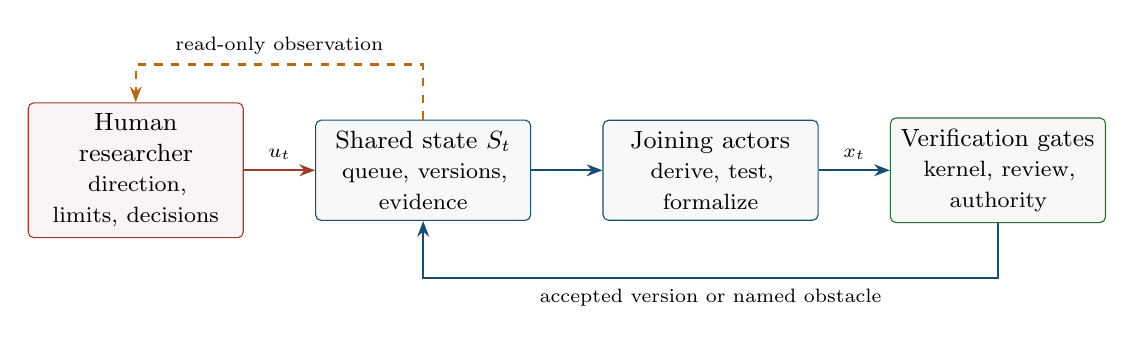
\begin{tikzpicture}[x=1cm,y=1cm,
 b/.style={draw=linkblue,rounded corners=2pt,fill=linkblue!4,text width=2.45cm,minimum height=1.1cm,align=center,font=\small,inner sep=4pt},
 a/.style={-{Stealth[length=2mm]},thick,draw=linkblue}]
\node[b,draw=humanred,fill=humanred!5] (h) at (0,0) {Human\\researcher\\\footnotesize direction, limits, decisions};
\node[b] (s) at (3.65,0) {Shared state $S_t$\\\footnotesize queue, versions, evidence};
\node[b] (w) at (7.3,0) {Joining actors\\\footnotesize derive, test, formalize};
\node[b,draw=reviewgreen,fill=reviewgreen!5] (g) at (10.95,0) {Verification gates\\\footnotesize kernel, review, authority};
\draw[a,draw=humanred] (h)--node[above,font=\scriptsize]{$u_t$}(s);
\draw[a] (s)--(w);
\draw[a] (w)--node[above,font=\scriptsize]{$x_t$}(g);
\draw[a] (g.south)--++(0,-0.7)-|node[pos=0.25,below,font=\scriptsize]{accepted version or named obstacle}(s.south);
\draw[a,dashed,draw=standorange] (s.north)--++(0,0.7)-|node[pos=0.25,above,font=\scriptsize]{read-only observation}(h.north);
\end{tikzpicture}
\caption{Human-guided supervisory control through external shared state. Both
verified advances and failed attempts remain visible to the human researcher,
while models and runtimes can be swapped without altering the scientific
objective, artifact identities or verification rules. Gate outcomes are kept
distinct: agreement among language models never promotes a statement to
kernel-checked status.}
\label{fig:model}
\end{figure}

\begin{table}[htbp]
\centering\small
\caption{Claim status and evidence standards used across drafts, living books
and internal review. Labels identify what kind of evidence backs a statement
rather than assigning an ordinal quality score.}
\label{tab:legend}
\begin{tabularx}{\linewidth}{@{}L{0.15\linewidth}L{0.30\linewidth}Y@{}}
\toprule
Status & Evidential basis & Meaning for readers and reviewers \\
\midrule
\textsc{lean} & Pinned frozen declaration and passing kernel check & Literal formal statement verified under declared definitions and axioms \\
\textsc{proved} & Complete human-readable proof with independent review & Checked prose argument whose formalization status is tracked separately \\
\textsc{classical} & Primary literature check with matched hypotheses & Verified attribution to an established external theorem \\
\textsc{hypothesis} & Explicit premise stated in the theorem & Declared assumption in a conditional result \\
\textsc{conjecture} & Precisely stated open target & Unresolved mathematical problem under active study \\
\textsc{programme} & Guiding direction with explicit missing links & Research agenda requiring further theorems or definitions \\
\textsc{refuted} & Quoted claim paired with an explicit counterexample & Falsified statement, retained with its repaired version when found \\
\bottomrule
\end{tabularx}
\end{table}

\subsection{Coupling Formal Verification to Readable Exposition}
\label{sec:architecture}
Tao's ``proof indigestion'' diagnosis \citep{tao2026age} highlights that
machine verification produces lasting science only when readers can inspect,
check and digest the argument. Our architecture therefore places the formal
verification hub at the centre of four coupled feedback loops
(Figure~\ref{fig:loop}). These loops connect exploratory derivation, bilingual
living exposition, claim-centered internal review (Section~\ref{sec:feedback})
and direct engagement with living domain scholars under the control boundaries
of Sections~\ref{sec:control} and~\ref{sec:harness}.

This coupling enforces a bidirectional discipline between formal code and
human prose. A manuscript claim may invoke a frozen Lean~4 theorem only after
its informal definitions, quantifiers and hypotheses are verified to match the
formal declaration; whenever review detects a discrepancy in that bridge, the
claim drops back to open or prose-only status until repaired. Conversely,
rewriting a machine-checked derivation into clean, self-contained prose often
exposes hidden assumptions or retrieves an already verified result from the
library, closing expository gaps without duplicating work.

\begin{figure}[htbp]
\centering
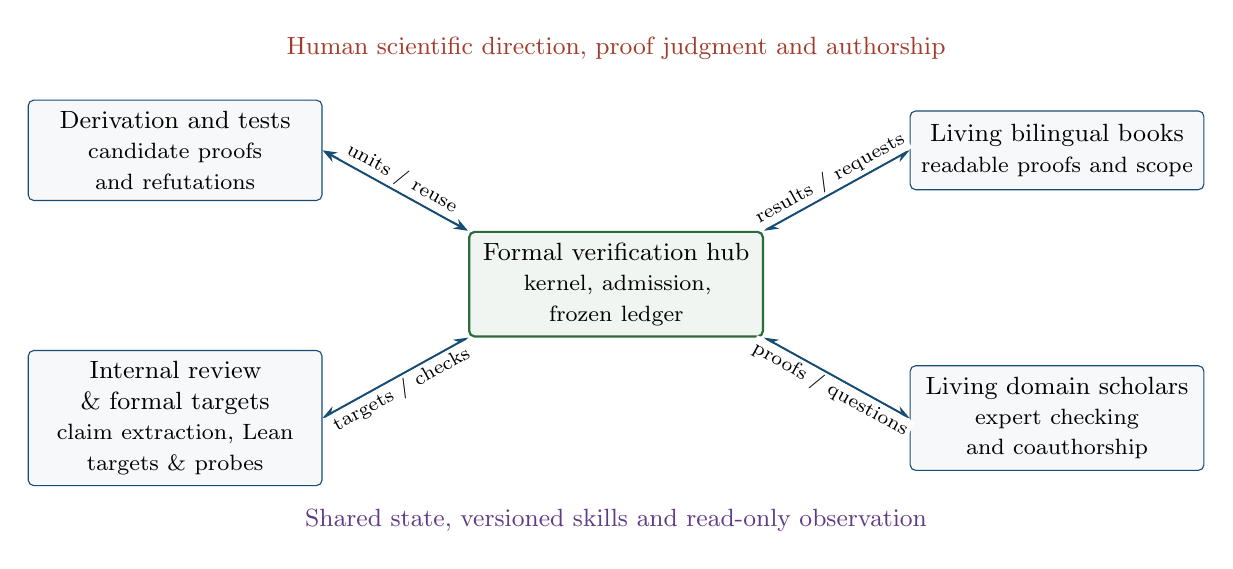
\begin{tikzpicture}[
 b/.style={draw=linkblue,fill=linkblue!4,rounded corners=2pt,text width=3.45cm,minimum height=1.0cm,align=center,font=\small,inner sep=4pt},
 hub/.style={b,draw=reviewgreen,fill=reviewgreen!7,thick},
 a/.style={{Stealth[length=1.8mm]}-{Stealth[length=1.8mm]},thick,draw=linkblue},
 lab/.style={font=\scriptsize,fill=white,inner sep=1pt}]
\node[hub] (k) at (0,0) {Formal verification hub\\\footnotesize kernel, admission, frozen ledger};
\node[b] (d) at (-5.6,1.7) {Derivation and tests\\\footnotesize candidate proofs and refutations};
\node[b] (b) at (5.6,1.7) {Living bilingual books\\\footnotesize readable proofs and scope};
\node[b] (m) at (-5.6,-1.7) {Internal review \& formal targets\\\footnotesize claim extraction, Lean targets \& probes};
\node[b] (e) at (5.6,-1.7) {Living domain scholars\\\footnotesize expert checking and coauthorship};
\draw[a] (d.east)--node[lab,sloped,above]{units / reuse}(k.north west);
\draw[a] (k.north east)--node[lab,sloped,above]{results / requests}(b.west);
\draw[a] (m.east)--node[lab,sloped,below]{targets / checks}(k.south west);
\draw[a] (k.south east)--node[lab,sloped,below]{proofs / questions}(e.west);
\node[font=\small,text=humanred] at (0,3.0) {Human scientific direction, proof judgment and authorship};
\node[font=\small,text=methodpurple] at (0,-3.0) {Shared state, versioned skills and read-only observation};
\end{tikzpicture}
\caption{Coupled research loops anchored around formal verification.
Claim-centered internal review feeds executable Lean~4 targets and private
kernel probes back to the hub, while living domain scholars bring independent
judgment of meaning, attribution and exposition. Bidirectional arrows indicate
exchanges of artifacts and questions across distinct standards of evidence.}
\label{fig:loop}
\end{figure}

\subsection{Preventing Synthetic Lemma Inflation}
\label{sec:admission}
A proof kernel certifies logical validity indiscriminately: it accepts a
trivial repackaging of Mathlib as readily as a deep theorem. Left unchecked,
automated theorem provers quickly generate ``formal slop'', producing dense
collections of synthetic lemmas that inflate repository counts without adding
mathematical substance. To separate formal validity from genuine contribution,
every new Lean~4 unit must clear four admission gates before its first freeze
(Box~\ref{box:antiinflation}). Here \emph{binding operations} refer to routine
instantiation, substitution, projection, recombination or normalization of
available library facts, and an \emph{escape witness} marks an intermediate
proof step beyond those operations.

\noindent\begin{minipage}{\linewidth}
\begin{protocol}{Four anti-inflation formal admission gates}
\label{box:antiinflation}
\begin{enumerate}
\item \textbf{Public preregistration before probing.} Record the exact target
statement, expected non-binding steps and admission basis in a public issue
before Lean probing begins; changing the target requires a fresh
preregistration.
\item \textbf{Library-first reuse.} Search the frozen knowledge base, pinned
Mathlib and admissible libraries first, importing existing theorems directly
rather than reproving them.
\item \textbf{No bind-only declarations.} Pure instantiation, substitution,
projection, recombination or normalization of existing facts cannot enter as a
standalone entry. Auxiliary lemmas must either serve an active proof path or
state the conclusion of a settled open problem.
\item \textbf{Escape witness or verbatim open-problem settlement.} First freeze
requires either a registered intermediate proposition escaping the declared
binding operations, or the verbatim settlement of a named literature problem
verified against the current literature. Finite enumeration enters only as a
typed refutation of a named claim. Escape definitions and templates are pinned
in Table~\ref{tab:repro}.
\end{enumerate}
\end{protocol}
\end{minipage}

An escape witness does not score mathematical importance; instead, it forces
every new unit to expose a non-trivial inferential step for human inspection.
Settling a literature problem likewise requires preserving the source
statement's quantifiers, boundary cases and current open status during
translation into Lean~4. Every admitted module must compile with zero
\code{sorry} placeholders and only whitelisted foundational axioms before its
statement identity and declarations are frozen; any later retraction propagates
along dependency edges to dependent claims. Because automated admission applies
identical rules to internal and external contributors, human mathematicians can
focus on whether each frozen theorem matches the prose claim and advances the
field.

\subsection{Open Model-Agnostic Harness and Cross-Family Critique}
\label{sec:harness}
Because reasoning models evolve rapidly, tying a long-horizon research
programme to a single proprietary runtime creates institutional lock-in. Our
harness therefore treats model and runtime independence as an interface
contract: general-purpose coding agents, specialized neural theorem provers and
human collaborators join by reading the same external state, adopting versioned
skill rules and submitting versioned artifacts to identical verification gates.
No actor's identity relaxes a formal check.

To counter the self-preference and blind spots documented in single-model
self-correction \citep{huang,panickssery,zheng2023judge}, the harness separates
authoring, fresh-context adversarial review and re-verified integration
(Box~\ref{box:delegate}; minimal prompts in Appendix~\ref{app:templates}).
Reviewers inspect a frozen snapshot cold, before seeing the author's list of
caveats. Delegating across distinct model families reduces correlated model
errors, while executable scripts and the Lean~4 kernel provide non-circular
adjudication. Because cross-family review alone cannot eliminate shared
training biases or translation slips, machine-checked obligations and living
human referees remain essential.

\noindent\begin{minipage}{\linewidth}
\begin{protocol}{Cross-family delegation and integration contract}
\label{box:delegate}
Each delegated task specifies an immutable source snapshot, exact hypotheses
and boundary conditions, asking for a complete proof, an explicit
counterexample or a partial theorem that pinpoints the remaining obstacle. The
returned bundle must pair a readable argument with checked primary citations,
executable verification scripts and explicit claim statuses. A fresh reviewer
from an independent model family then attacks every inference step, quantifier,
edge case and attribution before the integrating author independently rechecks
both prose and code against the same snapshot. Refuted claims are never quietly
discarded: their counterexamples and repaired formulations stay in the shared
record.
\end{protocol}
\end{minipage}

Execution isolation separates authoring privileges from read-only independent
review via scoped credentials and bounded sandboxes, while multi-machine
orchestration schedules formal builds within measured memory limits. Versioned
skill registries keep heterogeneous agents aligned on mathematical and
supervisory rules, and read-only progress monitors expose runs and failures to
human supervisors without granting any automated actor authority to publish or
make external commitments.

\subsection{Executable Review Obligations and Collaboration with Living Scholars}
\label{sec:feedback}
Prose-only automated peer review lowers the cost of generating objections
without lowering the cost of checking them. This asymmetry motivated Sun et
al.\ to propose an ``obligation threshold'' \citep{sun2026obligation}, while
benchmarks show that strong agentic reviewers still miss roughly a quarter of
injected errors \citep{stanford,nguyen2026review,scholarpeer}. Our internal
review loop addresses this gap by translating disputed manuscript claims into
executable Lean~4 verification targets alongside private kernel probes. After
source verification and dependency extraction isolate a manuscript's
load-bearing claims, any contested implication becomes a concrete formal
proposition whose hypotheses and conclusion can be inspected and tested. A
failed check returns an explicit gap, counterexample or weakened hypothesis to
the draft instead of an ambiguous prose critique. Across the live pipeline, 212
internally reviewed drafts register 1,480 explicit statements, 211 drafts link
to Lean~4 sources and seven curated executable targets accompany private kernel
probes; source linkage, registered claims and completed formal proofs are
tracked as distinct scopes. As this review and formal-target automation
matures, the loop aims to pair every resolved research line with a
self-contained manuscript and active external collaboration.

Two outward-facing channels turn machine-checked results into durable human
understanding. First, bilingual Chinese and English living books present each
research line in continuously updated, human-readable prose where formal
theorems link to pinned frozen declarations, prose-only arguments state their
exact status and open problems remain visibly open; corrections update the
statement and its dependent exposition in place. Second, direct scholarly
correspondence shares the original problem context, readable proof and exact
Lean~4 link with living domain experts, often the authors who posed the open
problem. Scholars challenge steps, refine hypotheses, identify missing
literature or enter joint authorship; opt-outs are honoured immediately, and
authorship, personal and publication decisions remain reserved to humans.
Section~\ref{sec:scholars} reports the resulting engagement and collaborative
outputs in full.

\section{Empirical Evaluation and Outcomes}
\label{sec:results}
To test whether keeping humans at the centre of a verification-centered loop
prevents scientific slop and proof indigestion, we present four complementary
empirical analyses: a 30-manuscript blinded benchmark scored across three
independent frontier model families alongside longitudinal arXiv revisions
(Section~\ref{sec:benchmark}), a controlled 20-claim mechanistic ablation of
prose review versus executable review obligations paired with a 24,925-PR
public admission-gate audit (Section~\ref{sec:ablation}), collaborative
outputs and scholar participation across the live programme
(Section~\ref{sec:scholars}), and a minute-by-minute instrumented 33-hour
research trace (Section~\ref{sec:case}).

\subsection{External Three-Cohort Blinded Benchmark and Longitudinal Collaboration}
\label{sec:benchmark}
\paragraph{Three-family external comparison ($N=30$, 90 evaluations).}
The blinded benchmark evaluates 30 real public manuscripts equally divided
among three cohorts ($n=10$ per cohort): autonomous AI-only studies from ten
distinct laboratories in \code{alphaXiv/AgentAlphaXiv}, contemporaneous
human-only arXiv preprints across six specialist subject classes, and
human-in-the-loop collaborative arXiv preprints matched to those exact six
classes. Three independent named frontier model families scored every
anonymized manuscript blindly under the same seven-item rubric: OpenAI Codex
(\code{gpt-6.1-sol} at \code{xhigh}), Anthropic Claude
(\code{claude-opus-5-5}) and Google Gemini (isolated fresh blind referees),
yielding 90 independent evaluations with strong three-family rank concordance
(Kendall $W=0.828$; pairwise Spearman $\rho=0.841$ between Claude and Gemini,
$\rho=0.769$ between Codex and Gemini, and $\rho=0.614$ between Codex and
Claude; all $p\le 3.0\times10^{-4}$).

Under every one of the three independent model families, human-in-the-loop
collaborative preprints achieve the highest mean overall score
(Table~\ref{tab:benchmark}; Figure~\ref{fig:benchmark}). Mean overall scores
for collaboration reach $8.25\pm0.68$ (Codex), $6.69\pm0.71$ (Claude) and
$8.32\pm0.56$ (Gemini), compared with $6.96\pm0.76$, $5.69\pm0.93$ and
$5.83\pm0.98$ for autonomous AI-only studies and $7.22\pm1.95$, $6.23\pm1.60$
and $7.23\pm2.36$ for contemporaneous human-only arXiv preprints (sample SDs
across ten papers per cohort). Collaborative manuscripts lead all six rubric
axes under both Codex and Gemini and lead correctness ($7.80$ versus $6.82$),
verification grounding ($7.34$ versus $6.65$), novelty and significance
($5.79$ versus $4.46$) and literature attribution ($6.90$ versus $5.57$) under
Claude's stricter calibration (where autonomous null-result studies score
slightly higher only on conservative claim calibration and uniform prose
polish). Consistent with the novelty and significance deficit reported in
autonomous agent societies \citep{societyai,oh2026slop}, autonomous AI-only
studies score lowest on novelty and significance under all three judges
($5.84$, $4.46$ and $5.15$), trailing collaborative papers by $+1.95$, $+1.33$
and $+2.67$ points.

Against the autonomous AI-only cohort, collaboration lifts overall scores by
$+1.29$ (Codex), $+1.00$ (Claude) and $+2.49$ (Gemini) points, winning 91/100,
71/100 and 98/100 cross-cohort pairwise comparisons (260 of 300 pooled
descriptive wins, or 86.7\%, with four ties). Exact two-sided permutation
tests over all $\binom{20}{10}=184{,}756$ assignments of the 20 manuscripts
yield $p=0.0012$ (Codex), $p=0.0149$ (Claude) and $p=0.000032$ (Gemini).
Against contemporaneous human-only arXiv preprints, mean differences are
$+1.03$, $+0.46$ and $+1.09$ ($p=0.1525$, $0.4321$ and $0.2233$), with
balanced category-matched head-to-head outcomes across the ten matched pairs
(6--4 under Codex, 5--5 under Claude, 4--6 under Gemini). Crucially, all three
independent judges unanimously flagged two unverified human-only preprints
containing fatal mathematical or physical errors: a singular-potential
\code{quant-ph} preprint (\arxiv{2610.21044v1}; scored 4.4, 3.5 and 3.2) and
an operator-splitting \code{math.CO} preprint (\arxiv{2611.00145v1}, whose
central Hopf-algebra theorem miscounts tree acyclic orientations as 1 instead
of $2^{|E|}$; scored 3.0, 3.5 and 2.8). Removing those two fatal-error papers
leaves the eight sound human-only preprints at $8.10\pm0.57$ (Codex),
$6.91\pm0.80$ (Claude) and $8.29\pm0.88$ (Gemini), statistically
indistinguishable from our ten collaborative papers ($8.25\pm0.68$,
$6.69\pm0.71$ and $8.32\pm0.56$). By contrast, the single human-only preprint
carrying a Lean~4 formalization (\arxiv{2611.00153v1}) ranked first in its
cohort under Claude (8.0) and Gemini (9.2) and second under Codex (8.1).
Verification-centered collaboration thus matches strong human arXiv research
while compressing full-sample overall dispersion 2.3- to 4.2-fold (SD 0.68,
0.71 and 0.56 versus 1.95, 1.60 and 2.36) and eliminating the unverified
low-rigor tail across all ten papers.

% Generated by scripts/render_benchmark.py from archived benchmark JSON.
\begin{table}[htbp]
\centering\scriptsize
\setlength{\tabcolsep}{2.2pt}
\caption{External three-cohort benchmark across three named model families and longitudinal revisions. A: ten-point scores (mean $\pm$ sample SD across ten manuscripts per cohort; 90 blinded evaluations total; Kendall concordance $W=0.828$). B: full-document structure and verification counts ($n=10$ per cohort). C: separate, version-blinded public arXiv revision study (overall scores, changes and elapsed calendar days). AI: autonomous AgentAlphaXiv; H: contemporaneous human-only arXiv; H+AI: human-in-the-loop collaboration.}
\label{tab:benchmark}
\textbf{A. Three-family blinded cohort scoring: 30 manuscripts, 90 evaluations ($n=10$ per cohort)}\par\smallskip
\begin{tabularx}{\linewidth}{@{}Yccccccccc@{}}
\toprule & \multicolumn{3}{c}{Codex (\code{gpt-6.1-sol})} & \multicolumn{3}{c}{Claude (\code{opus-5-5})} & \multicolumn{3}{c}{Google Gemini} \\
\cmidrule(lr){2-4}\cmidrule(lr){5-7}\cmidrule(l){8-10}
Axis & AI & H & H+AI & AI & H & H+AI & AI & H & H+AI \\ \midrule
Correctness and rigor & $7.94\pm0.82$ & $7.40\pm2.13$ & $8.66\pm0.72$ & $6.82\pm0.26$ & $6.85\pm1.73$ & $7.80\pm0.57$ & $6.57\pm1.10$ & $7.41\pm2.49$ & $8.93\pm0.54$ \\
Claim calibration & $8.60\pm1.10$ & $7.75\pm2.13$ & $8.86\pm0.85$ & $8.10\pm0.69$ & $6.82\pm1.99$ & $7.89\pm0.86$ & $8.62\pm0.45$ & $7.57\pm2.37$ & $9.00\pm0.52$ \\
Verification grounding & $7.57\pm0.66$ & $6.97\pm1.92$ & $8.48\pm0.80$ & $6.65\pm0.49$ & $5.99\pm1.65$ & $7.34\pm1.06$ & $7.23\pm0.66$ & $7.02\pm2.34$ & $8.88\pm0.51$ \\
Novelty and significance & $5.84\pm1.34$ & $7.31\pm1.55$ & $7.79\pm0.78$ & $4.46\pm1.23$ & $5.75\pm1.46$ & $5.79\pm0.95$ & $5.15\pm1.34$ & $7.20\pm2.31$ & $7.82\pm0.79$ \\
Literature attribution & $7.19\pm1.61$ & $7.91\pm1.08$ & $8.38\pm0.88$ & $5.57\pm1.49$ & $6.09\pm1.61$ & $6.90\pm0.70$ & $6.56\pm1.91$ & $7.84\pm1.77$ & $8.64\pm0.33$ \\
Clarity and exposition & $8.33\pm0.30$ & $7.84\pm1.15$ & $8.48\pm0.49$ & $7.22\pm0.30$ & $6.83\pm1.33$ & $6.85\pm0.79$ & $7.62\pm0.49$ & $7.77\pm1.73$ & $8.49\pm0.76$ \\
\textbf{Overall} & $6.96\pm0.76$ & $7.22\pm1.95$ & $8.25\pm0.68$ & $5.69\pm0.93$ & $6.23\pm1.60$ & $6.69\pm0.71$ & $5.83\pm0.98$ & $7.23\pm2.36$ & $8.32\pm0.56$ \\
\midrule
H+AI vs.\ AI (184,756 perm.) & \multicolumn{3}{c}{91/100 wins; $p=0.0012$} & \multicolumn{3}{c}{71/100 wins; $p=0.0149$} & \multicolumn{3}{c}{98/100 wins; $p=0.000032$} \\
\bottomrule\end{tabularx}
\par\vspace{7pt}
\textbf{B. Full-document structure and verification artifacts ($n=10$ per cohort)}\par\smallskip
\setlength{\tabcolsep}{4pt}
\begin{tabularx}{\linewidth}{@{}Yccc@{}}
\toprule Metric & AI & H & H+AI \\ \midrule
Pages, mean (median) & 12.2 (11.5) & 19.6 (18.5) & 26.7 (17.5) \\
Theorem / lemma / proposition blocks, total (mean) & 1 (0.1) & 119 (11.9) & 165 (16.5) \\
Proof blocks, total (mean) & 1 (0.1) & 84 (8.4) & 139 (13.9) \\
Papers reporting formal or certified checks & 0/10 & 1/10 & 10/10 \\
Verification-related text mentions, total & 3 & 19 & 80 \\
References, median & 20 & 20 & 18 \\
\bottomrule\end{tabularx}
\smallskip
\begin{minipage}{\linewidth}\scriptsize Verification artifacts in H+AI span Lean~4 proofs, DRAT certificates, 192-bit Arb interval enclosures and exact polynomial, rational or exhaustive certificates across all ten manuscripts. The single formally verified human-only preprint (\arxiv{2611.00153v1}, Lean~4) ranked highest in its cohort under Claude (8.0) and Gemini (9.2) and second under Codex (8.1).\end{minipage}
\par\vspace{7pt}
\textbf{C. Longitudinal external collaboration: public v1$\to$vK}\par\smallskip
\begin{tabularx}{\linewidth}{@{}Yccccc@{}}
\toprule & & \multicolumn{2}{c}{Judge 1} & \multicolumn{2}{c}{Judge 2} \\
\cmidrule(lr){3-4}\cmidrule(l){5-6}
arXiv ID and versions & Days & v1 $\to$ vK & $\Delta$ & v1 $\to$ vK & $\Delta$ \\ \midrule
\arxiv{2610.05623} v1$\to$v2 & 30 & $3.8\to8.0$ & $+4.2$ & $4.7\to8.9$ & $+4.2$ \\
\arxiv{2609.09753} v1$\to$v3 & 41 & $6.6\to8.0$ & $+1.4$ & $5.6\to8.5$ & $+2.9$ \\
\arxiv{2609.25128} v1$\to$v4 & 20 & $5.9\to7.0$ & $+1.1$ & $6.4\to8.5$ & $+2.1$ \\
\arxiv{2610.18816} v1$\to$v2 & 2 & $8.2\to8.2$ & $0.0$ & $8.7\to8.5$ & $-0.2$ \\
\arxiv{2610.39941} v1$\to$v2 & 12 & $7.2\to7.2$ & $0.0$ & $8.0\to8.1$ & $+0.1$ \\
\bottomrule\end{tabularx}
\smallskip
\begin{minipage}{\linewidth}\scriptsize The final two rows are minor-edit negative controls. Panels A and C use separate scoring contexts; their absolute scores are not interchangeable.\end{minipage}
\end{table}

% Generated by scripts/render_benchmark.py; coordinates are archived JSON scores.
\begin{figure}[htbp]
\centering
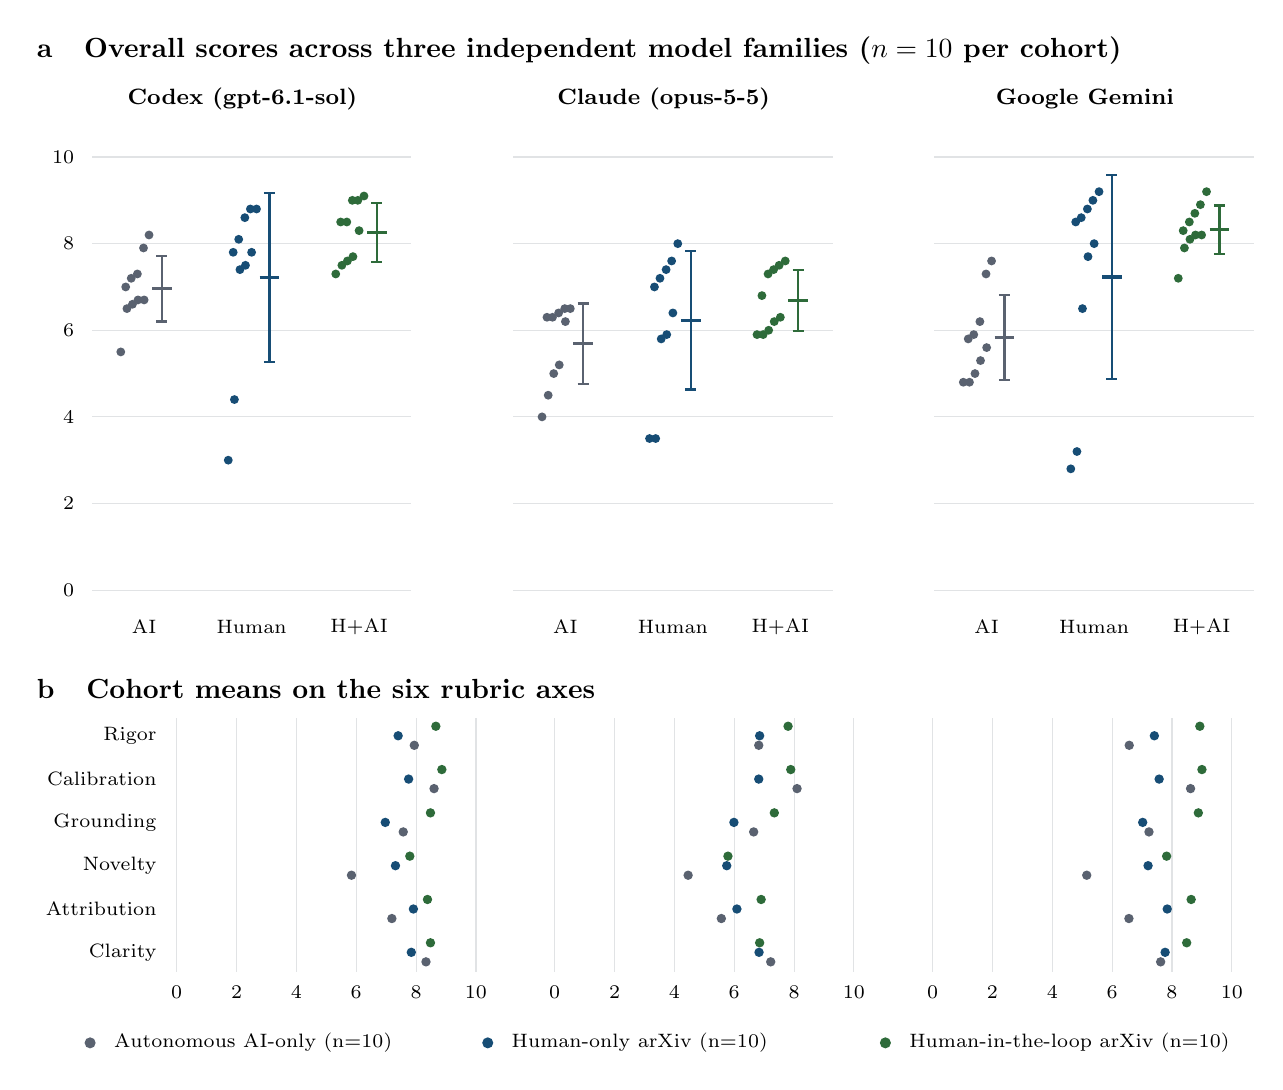
\begin{tikzpicture}[font=\small]
\node[anchor=west,font=\bfseries] at (-0.55,6.85) {a\quad Overall scores across three independent model families ($n=10$ per cohort)};
\begin{scope}[xshift=0.00cm,x=0.78cm,y=0.55cm]
\node[font=\footnotesize\bfseries] at (2.8,11.35) {Codex (gpt-6.1-sol)};
\draw[planegray!18] (0.35,0)--(5.55,0);
\node[anchor=east,font=\scriptsize] at (0.22,0) {0};
\draw[planegray!18] (0.35,2)--(5.55,2);
\node[anchor=east,font=\scriptsize] at (0.22,2) {2};
\draw[planegray!18] (0.35,4)--(5.55,4);
\node[anchor=east,font=\scriptsize] at (0.22,4) {4};
\draw[planegray!18] (0.35,6)--(5.55,6);
\node[anchor=east,font=\scriptsize] at (0.22,6) {6};
\draw[planegray!18] (0.35,8)--(5.55,8);
\node[anchor=east,font=\scriptsize] at (0.22,8) {8};
\draw[planegray!18] (0.35,10)--(5.55,10);
\node[anchor=east,font=\scriptsize] at (0.22,10) {10};
\fill[planegray] (0.82,5.50) circle (1.6pt);
\fill[planegray] (0.92,6.50) circle (1.6pt);
\fill[planegray] (1.01,6.60) circle (1.6pt);
\fill[planegray] (1.10,6.70) circle (1.6pt);
\fill[planegray] (1.20,6.70) circle (1.6pt);
\fill[planegray] (0.90,7.00) circle (1.6pt);
\fill[planegray] (0.99,7.20) circle (1.6pt);
\fill[planegray] (1.09,7.30) circle (1.6pt);
\fill[planegray] (1.19,7.90) circle (1.6pt);
\fill[planegray] (1.28,8.20) circle (1.6pt);
\draw[planegray,thick] (1.49,6.20)--(1.49,7.72);
\draw[planegray,thick] (1.40,6.20)--(1.58,6.20) (1.40,7.72)--(1.58,7.72);
\draw[planegray,very thick] (1.33,6.96)--(1.65,6.96);
\node[font=\scriptsize,align=center] at (1.20,-0.85) {AI};
\fill[linkblue] (2.57,3.00) circle (1.6pt);
\fill[linkblue] (2.67,4.40) circle (1.6pt);
\fill[linkblue] (2.76,7.40) circle (1.6pt);
\fill[linkblue] (2.85,7.50) circle (1.6pt);
\fill[linkblue] (2.95,7.80) circle (1.6pt);
\fill[linkblue] (2.65,7.80) circle (1.6pt);
\fill[linkblue] (2.74,8.10) circle (1.6pt);
\fill[linkblue] (2.84,8.60) circle (1.6pt);
\fill[linkblue] (2.93,8.80) circle (1.6pt);
\fill[linkblue] (3.03,8.80) circle (1.6pt);
\draw[linkblue,thick] (3.24,5.27)--(3.24,9.17);
\draw[linkblue,thick] (3.15,5.27)--(3.33,5.27) (3.15,9.17)--(3.33,9.17);
\draw[linkblue,very thick] (3.08,7.22)--(3.40,7.22);
\node[font=\scriptsize,align=center] at (2.95,-0.85) {Human};
\fill[reviewgreen] (4.32,7.30) circle (1.6pt);
\fill[reviewgreen] (4.42,7.50) circle (1.6pt);
\fill[reviewgreen] (4.51,7.60) circle (1.6pt);
\fill[reviewgreen] (4.60,7.70) circle (1.6pt);
\fill[reviewgreen] (4.70,8.30) circle (1.6pt);
\fill[reviewgreen] (4.40,8.50) circle (1.6pt);
\fill[reviewgreen] (4.50,8.50) circle (1.6pt);
\fill[reviewgreen] (4.59,9.00) circle (1.6pt);
\fill[reviewgreen] (4.68,9.00) circle (1.6pt);
\fill[reviewgreen] (4.78,9.10) circle (1.6pt);
\draw[reviewgreen,thick] (4.99,7.57)--(4.99,8.93);
\draw[reviewgreen,thick] (4.90,7.57)--(5.08,7.57) (4.90,8.93)--(5.08,8.93);
\draw[reviewgreen,very thick] (4.83,8.25)--(5.15,8.25);
\node[font=\scriptsize,align=center] at (4.70,-0.85) {H+AI};
\end{scope}
\begin{scope}[xshift=5.35cm,x=0.78cm,y=0.55cm]
\node[font=\footnotesize\bfseries] at (2.8,11.35) {Claude (opus-5-5)};
\draw[planegray!18] (0.35,0)--(5.55,0);
\draw[planegray!18] (0.35,2)--(5.55,2);
\draw[planegray!18] (0.35,4)--(5.55,4);
\draw[planegray!18] (0.35,6)--(5.55,6);
\draw[planegray!18] (0.35,8)--(5.55,8);
\draw[planegray!18] (0.35,10)--(5.55,10);
\fill[planegray] (0.82,4.00) circle (1.6pt);
\fill[planegray] (0.92,4.50) circle (1.6pt);
\fill[planegray] (1.01,5.00) circle (1.6pt);
\fill[planegray] (1.10,5.20) circle (1.6pt);
\fill[planegray] (1.20,6.20) circle (1.6pt);
\fill[planegray] (0.90,6.30) circle (1.6pt);
\fill[planegray] (0.99,6.30) circle (1.6pt);
\fill[planegray] (1.09,6.40) circle (1.6pt);
\fill[planegray] (1.19,6.50) circle (1.6pt);
\fill[planegray] (1.28,6.50) circle (1.6pt);
\draw[planegray,thick] (1.49,4.76)--(1.49,6.62);
\draw[planegray,thick] (1.40,4.76)--(1.58,4.76) (1.40,6.62)--(1.58,6.62);
\draw[planegray,very thick] (1.33,5.69)--(1.65,5.69);
\node[font=\scriptsize,align=center] at (1.20,-0.85) {AI};
\fill[linkblue] (2.57,3.50) circle (1.6pt);
\fill[linkblue] (2.67,3.50) circle (1.6pt);
\fill[linkblue] (2.76,5.80) circle (1.6pt);
\fill[linkblue] (2.85,5.90) circle (1.6pt);
\fill[linkblue] (2.95,6.40) circle (1.6pt);
\fill[linkblue] (2.65,7.00) circle (1.6pt);
\fill[linkblue] (2.74,7.20) circle (1.6pt);
\fill[linkblue] (2.84,7.40) circle (1.6pt);
\fill[linkblue] (2.93,7.60) circle (1.6pt);
\fill[linkblue] (3.03,8.00) circle (1.6pt);
\draw[linkblue,thick] (3.24,4.63)--(3.24,7.83);
\draw[linkblue,thick] (3.15,4.63)--(3.33,4.63) (3.15,7.83)--(3.33,7.83);
\draw[linkblue,very thick] (3.08,6.23)--(3.40,6.23);
\node[font=\scriptsize,align=center] at (2.95,-0.85) {Human};
\fill[reviewgreen] (4.32,5.90) circle (1.6pt);
\fill[reviewgreen] (4.42,5.90) circle (1.6pt);
\fill[reviewgreen] (4.51,6.00) circle (1.6pt);
\fill[reviewgreen] (4.60,6.20) circle (1.6pt);
\fill[reviewgreen] (4.70,6.30) circle (1.6pt);
\fill[reviewgreen] (4.40,6.80) circle (1.6pt);
\fill[reviewgreen] (4.50,7.30) circle (1.6pt);
\fill[reviewgreen] (4.59,7.40) circle (1.6pt);
\fill[reviewgreen] (4.68,7.50) circle (1.6pt);
\fill[reviewgreen] (4.78,7.60) circle (1.6pt);
\draw[reviewgreen,thick] (4.99,5.98)--(4.99,7.40);
\draw[reviewgreen,thick] (4.90,5.98)--(5.08,5.98) (4.90,7.40)--(5.08,7.40);
\draw[reviewgreen,very thick] (4.83,6.69)--(5.15,6.69);
\node[font=\scriptsize,align=center] at (4.70,-0.85) {H+AI};
\end{scope}
\begin{scope}[xshift=10.70cm,x=0.78cm,y=0.55cm]
\node[font=\footnotesize\bfseries] at (2.8,11.35) {Google Gemini};
\draw[planegray!18] (0.35,0)--(5.55,0);
\draw[planegray!18] (0.35,2)--(5.55,2);
\draw[planegray!18] (0.35,4)--(5.55,4);
\draw[planegray!18] (0.35,6)--(5.55,6);
\draw[planegray!18] (0.35,8)--(5.55,8);
\draw[planegray!18] (0.35,10)--(5.55,10);
\fill[planegray] (0.82,4.80) circle (1.6pt);
\fill[planegray] (0.92,4.80) circle (1.6pt);
\fill[planegray] (1.01,5.00) circle (1.6pt);
\fill[planegray] (1.10,5.30) circle (1.6pt);
\fill[planegray] (1.20,5.60) circle (1.6pt);
\fill[planegray] (0.90,5.80) circle (1.6pt);
\fill[planegray] (0.99,5.90) circle (1.6pt);
\fill[planegray] (1.09,6.20) circle (1.6pt);
\fill[planegray] (1.19,7.30) circle (1.6pt);
\fill[planegray] (1.28,7.60) circle (1.6pt);
\draw[planegray,thick] (1.49,4.85)--(1.49,6.81);
\draw[planegray,thick] (1.40,4.85)--(1.58,4.85) (1.40,6.81)--(1.58,6.81);
\draw[planegray,very thick] (1.33,5.83)--(1.65,5.83);
\node[font=\scriptsize,align=center] at (1.20,-0.85) {AI};
\fill[linkblue] (2.57,2.80) circle (1.6pt);
\fill[linkblue] (2.67,3.20) circle (1.6pt);
\fill[linkblue] (2.76,6.50) circle (1.6pt);
\fill[linkblue] (2.85,7.70) circle (1.6pt);
\fill[linkblue] (2.95,8.00) circle (1.6pt);
\fill[linkblue] (2.65,8.50) circle (1.6pt);
\fill[linkblue] (2.74,8.60) circle (1.6pt);
\fill[linkblue] (2.84,8.80) circle (1.6pt);
\fill[linkblue] (2.93,9.00) circle (1.6pt);
\fill[linkblue] (3.03,9.20) circle (1.6pt);
\draw[linkblue,thick] (3.24,4.87)--(3.24,9.59);
\draw[linkblue,thick] (3.15,4.87)--(3.33,4.87) (3.15,9.59)--(3.33,9.59);
\draw[linkblue,very thick] (3.08,7.23)--(3.40,7.23);
\node[font=\scriptsize,align=center] at (2.95,-0.85) {Human};
\fill[reviewgreen] (4.32,7.20) circle (1.6pt);
\fill[reviewgreen] (4.42,7.90) circle (1.6pt);
\fill[reviewgreen] (4.51,8.10) circle (1.6pt);
\fill[reviewgreen] (4.60,8.20) circle (1.6pt);
\fill[reviewgreen] (4.70,8.20) circle (1.6pt);
\fill[reviewgreen] (4.40,8.30) circle (1.6pt);
\fill[reviewgreen] (4.50,8.50) circle (1.6pt);
\fill[reviewgreen] (4.59,8.70) circle (1.6pt);
\fill[reviewgreen] (4.68,8.90) circle (1.6pt);
\fill[reviewgreen] (4.78,9.20) circle (1.6pt);
\draw[reviewgreen,thick] (4.99,7.76)--(4.99,8.88);
\draw[reviewgreen,thick] (4.90,7.76)--(5.08,7.76) (4.90,8.88)--(5.08,8.88);
\draw[reviewgreen,very thick] (4.83,8.32)--(5.15,8.32);
\node[font=\scriptsize,align=center] at (4.70,-0.85) {H+AI};
\end{scope}
\node[anchor=west,font=\bfseries] at (-0.55,-1.25) {b\quad Cohort means on the six rubric axes};
\begin{scope}[xshift=1.35cm,yshift=-1.85cm,x=0.38cm,y=0.55cm]
\draw[planegray!18] (0,-5.45)--(0,0.4);
\node[below,font=\scriptsize] at (0,-5.55) {0};
\draw[planegray!18] (2,-5.45)--(2,0.4);
\node[below,font=\scriptsize] at (2,-5.55) {2};
\draw[planegray!18] (4,-5.45)--(4,0.4);
\node[below,font=\scriptsize] at (4,-5.55) {4};
\draw[planegray!18] (6,-5.45)--(6,0.4);
\node[below,font=\scriptsize] at (6,-5.55) {6};
\draw[planegray!18] (8,-5.45)--(8,0.4);
\node[below,font=\scriptsize] at (8,-5.55) {8};
\draw[planegray!18] (10,-5.45)--(10,0.4);
\node[below,font=\scriptsize] at (10,-5.55) {10};
\node[anchor=east,font=\scriptsize] at (-0.35,0) {Rigor};
\fill[planegray] (7.94,-0.22) circle (1.7pt);
\fill[linkblue] (7.40,0.00) circle (1.7pt);
\fill[reviewgreen] (8.66,0.22) circle (1.7pt);
\node[anchor=east,font=\scriptsize] at (-0.35,-1) {Calibration};
\fill[planegray] (8.60,-1.22) circle (1.7pt);
\fill[linkblue] (7.75,-1.00) circle (1.7pt);
\fill[reviewgreen] (8.86,-0.78) circle (1.7pt);
\node[anchor=east,font=\scriptsize] at (-0.35,-2) {Grounding};
\fill[planegray] (7.57,-2.22) circle (1.7pt);
\fill[linkblue] (6.97,-2.00) circle (1.7pt);
\fill[reviewgreen] (8.48,-1.78) circle (1.7pt);
\node[anchor=east,font=\scriptsize] at (-0.35,-3) {Novelty};
\fill[planegray] (5.84,-3.22) circle (1.7pt);
\fill[linkblue] (7.31,-3.00) circle (1.7pt);
\fill[reviewgreen] (7.79,-2.78) circle (1.7pt);
\node[anchor=east,font=\scriptsize] at (-0.35,-4) {Attribution};
\fill[planegray] (7.19,-4.22) circle (1.7pt);
\fill[linkblue] (7.91,-4.00) circle (1.7pt);
\fill[reviewgreen] (8.38,-3.78) circle (1.7pt);
\node[anchor=east,font=\scriptsize] at (-0.35,-5) {Clarity};
\fill[planegray] (8.33,-5.22) circle (1.7pt);
\fill[linkblue] (7.84,-5.00) circle (1.7pt);
\fill[reviewgreen] (8.48,-4.78) circle (1.7pt);
\end{scope}
\begin{scope}[xshift=6.15cm,yshift=-1.85cm,x=0.38cm,y=0.55cm]
\draw[planegray!18] (0,-5.45)--(0,0.4);
\node[below,font=\scriptsize] at (0,-5.55) {0};
\draw[planegray!18] (2,-5.45)--(2,0.4);
\node[below,font=\scriptsize] at (2,-5.55) {2};
\draw[planegray!18] (4,-5.45)--(4,0.4);
\node[below,font=\scriptsize] at (4,-5.55) {4};
\draw[planegray!18] (6,-5.45)--(6,0.4);
\node[below,font=\scriptsize] at (6,-5.55) {6};
\draw[planegray!18] (8,-5.45)--(8,0.4);
\node[below,font=\scriptsize] at (8,-5.55) {8};
\draw[planegray!18] (10,-5.45)--(10,0.4);
\node[below,font=\scriptsize] at (10,-5.55) {10};
\fill[planegray] (6.82,-0.22) circle (1.7pt);
\fill[linkblue] (6.85,0.00) circle (1.7pt);
\fill[reviewgreen] (7.80,0.22) circle (1.7pt);
\fill[planegray] (8.10,-1.22) circle (1.7pt);
\fill[linkblue] (6.82,-1.00) circle (1.7pt);
\fill[reviewgreen] (7.89,-0.78) circle (1.7pt);
\fill[planegray] (6.65,-2.22) circle (1.7pt);
\fill[linkblue] (5.99,-2.00) circle (1.7pt);
\fill[reviewgreen] (7.34,-1.78) circle (1.7pt);
\fill[planegray] (4.46,-3.22) circle (1.7pt);
\fill[linkblue] (5.75,-3.00) circle (1.7pt);
\fill[reviewgreen] (5.79,-2.78) circle (1.7pt);
\fill[planegray] (5.57,-4.22) circle (1.7pt);
\fill[linkblue] (6.09,-4.00) circle (1.7pt);
\fill[reviewgreen] (6.90,-3.78) circle (1.7pt);
\fill[planegray] (7.22,-5.22) circle (1.7pt);
\fill[linkblue] (6.83,-5.00) circle (1.7pt);
\fill[reviewgreen] (6.85,-4.78) circle (1.7pt);
\end{scope}
\begin{scope}[xshift=10.95cm,yshift=-1.85cm,x=0.38cm,y=0.55cm]
\draw[planegray!18] (0,-5.45)--(0,0.4);
\node[below,font=\scriptsize] at (0,-5.55) {0};
\draw[planegray!18] (2,-5.45)--(2,0.4);
\node[below,font=\scriptsize] at (2,-5.55) {2};
\draw[planegray!18] (4,-5.45)--(4,0.4);
\node[below,font=\scriptsize] at (4,-5.55) {4};
\draw[planegray!18] (6,-5.45)--(6,0.4);
\node[below,font=\scriptsize] at (6,-5.55) {6};
\draw[planegray!18] (8,-5.45)--(8,0.4);
\node[below,font=\scriptsize] at (8,-5.55) {8};
\draw[planegray!18] (10,-5.45)--(10,0.4);
\node[below,font=\scriptsize] at (10,-5.55) {10};
\fill[planegray] (6.57,-0.22) circle (1.7pt);
\fill[linkblue] (7.41,0.00) circle (1.7pt);
\fill[reviewgreen] (8.93,0.22) circle (1.7pt);
\fill[planegray] (8.62,-1.22) circle (1.7pt);
\fill[linkblue] (7.57,-1.00) circle (1.7pt);
\fill[reviewgreen] (9.00,-0.78) circle (1.7pt);
\fill[planegray] (7.23,-2.22) circle (1.7pt);
\fill[linkblue] (7.02,-2.00) circle (1.7pt);
\fill[reviewgreen] (8.88,-1.78) circle (1.7pt);
\fill[planegray] (5.15,-3.22) circle (1.7pt);
\fill[linkblue] (7.20,-3.00) circle (1.7pt);
\fill[reviewgreen] (7.82,-2.78) circle (1.7pt);
\fill[planegray] (6.56,-4.22) circle (1.7pt);
\fill[linkblue] (7.84,-4.00) circle (1.7pt);
\fill[reviewgreen] (8.64,-3.78) circle (1.7pt);
\fill[planegray] (7.62,-5.22) circle (1.7pt);
\fill[linkblue] (7.77,-5.00) circle (1.7pt);
\fill[reviewgreen] (8.49,-4.78) circle (1.7pt);
\end{scope}
\fill[planegray] (0.25,-5.75) circle (2pt);
\node[anchor=west,font=\scriptsize] at (0.43,-5.75) {Autonomous AI-only (n=10)};
\fill[linkblue] (5.30,-5.75) circle (2pt);
\node[anchor=west,font=\scriptsize] at (5.48,-5.75) {Human-only arXiv (n=10)};
\fill[reviewgreen] (10.35,-5.75) circle (2pt);
\node[anchor=west,font=\scriptsize] at (10.53,-5.75) {Human-in-the-loop arXiv (n=10)};
\end{tikzpicture}
\caption{Three-cohort external benchmark across three independent model families ($N=30$ public manuscripts, 90 blinded evaluations). Panel a displays every overall score alongside cohort means (thick crossbars) and sample SDs (capped bars) on the full 0--10 scale, showing both the systematic margin over autonomous AI-only studies and the 2.3- to 4.2-fold dispersion compression relative to unverified human preprints (whose low tail reflects two fatal-error papers independently flagged by all three judges). Panel b shows cohort means on each rubric axis. Three-family rank concordance across all 30 manuscripts is Kendall $W=0.828$. Dots represent blind manuscript judgments rather than kernel proofs; exact values and permutation tests appear in Table~\ref{tab:benchmark}.}
\label{fig:benchmark}
\end{figure}


\paragraph{Deductive depth and machine-checked backing.}
Full-document structural extraction confirms that these blind judge margins
reflect deep deductive grounding rather than surface polish
(Table~\ref{tab:benchmark}B). Across the ten autonomous AI-only studies (mean
12.2 pages, median 20 references, many citing unpublished internal agent
notes), the entire cohort contains only a single theorem, lemma or proposition
block and a single proof block combined, with zero formal or certified
mathematical checks (0/10). The ten human-only arXiv preprints (mean 19.6
pages, median 20 references) contain 119 statement blocks and 84 proof blocks,
with one paper (1/10, \arxiv{2611.00153v1}) carrying Lean~4 formalization.
The ten collaborative preprints (mean 26.7 pages, median 17.5 pages, median 18
references) contain 165 statement blocks and 139 proof blocks, and all ten
(10/10) carry explicit formal or certified verification spanning Lean~4 proofs,
independently checked DRAT certificates, outward-rounded 192-bit Arb interval
enclosures and exact polynomial, rational or exhaustive finite certificates
(80 verification-related mentions versus 19 in human-only arXiv and three
passing mentions in autonomous studies). Nine of the ten collaborative papers
are coauthored with external academics (and all ten human-only preprints are
externally authored), whereas no autonomous study lists an external academic
coauthor.

\paragraph{Longitudinal external arXiv revisions.}
To observe how human-AI verification changes an existing paper over time, we
conducted a separate version-blinded paired evaluation across five public
multi-version arXiv trajectories ($\text{v1}\to\text{v}K$;
Table~\ref{tab:benchmark}C), drawn from a ten-pair revision study whose five
internal drafts are omitted to keep the evaluation strictly external. Version
order was hidden via counterbalanced A/B randomization (seed 20261126), headers
and dates were stripped, texts were capped at 36,000 characters, and two blind
cross-family referees scored each version independently without the key.

The clearest inflection occurs in \arxiv{2610.05623v1} (4 October) to
\arxiv{2610.05623v2} (3 November), where a solo physicist's preprint entered
collaboration and became a coauthored manuscript within 30 days. Both judges
independently record $+4.2$ overall and $+5.2$ correctness gains (rising from
3.8 to 8.0 and 4.7 to 8.9 overall), pinpointing the same mathematical repairs:
a missing factor of two in Wigner inversion and contradictory vacuum coherence
prefactors (four versus two), alongside expanded positivity, complete inertia
and convergence theorems (pages rising from 10 to 15, theorem blocks from 1 to
4, proof blocks from 2 to 4 and references from 41 to 51). Substantive
collaborative revisions in \arxiv{2609.09753v1}$\to$\arxiv{2609.09753v3} (41
days, 9 September--20 October) and
\arxiv{2609.25128v1}$\to$\arxiv{2609.25128v4} (20 days, 20 September--10
October) similarly lift overall scores by $+1.4/+2.9$ (pages $9\to15$,
statements $15\to20$, proofs $10\to16$) and $+1.1/+2.1$ (pages $13\to19$,
statements $18\to30$, proofs $14\to26$). By contrast, two minor-edit controls,
\arxiv{2610.18816v2} (two days, moving an inline Hahn--Banach step to an
appendix citation) and \arxiv{2610.39941v2} (12 days, clarifying a definition
before use), produce near-zero deltas ($0.0/-0.2$ and $0.0/+0.1$), confirming
that judges reward substantive mathematical repairs rather than later versions
per se.

\paragraph{Sampling, blinding and reproducibility protocol.}
The autonomous AI-only cohort comprises ten studies drawn deterministically
from the 881 eligible studies in \code{alphaXiv/AgentAlphaXiv}
\citep{societyai} by ranking mathematical and theoretical keyword coverage
without consulting referee scores and selecting the top ten from distinct
laboratories (Labs~1, 2, 5, 7, 8, 11, 12, 13, 14 and 18). The collaborative
cohort comprises ten October--November 2026 specialist-category preprints
(excluding general mathematics \code{math.GM}) spanning six primary classes
(\code{quant-ph} $\times 3$, \code{math.CO} $\times 3$, \code{math.NT},
\code{cs.IT}, \code{math.GR} and \code{cs.FL}). Contemporaneous human-only
comparators are the first eligible non-collaborator regular research preprints
returned in ascending arXiv listing order from October--November 2026 in the
exact same six primary classes (full identities and PDF digests in
Appendix~\ref{app:repro} and the archived manifest). All 30 extracted texts
were randomized under fixed seeds (20261127 for \code{ext_01}--\code{ext_15};
2026112702 for \code{ext_16}--\code{ext_30}), stripped of authors,
affiliations, running headers, address footers, arXiv stamps, URLs, emails,
platform names and agent tags, and capped at 36,000 characters with an explicit
truncation marker where needed. All selection, blinding, scoring and
permutation-test scripts, together with every named-model JSON response, are
archived in \code{scripts/benchmark/} and \code{data/benchmark/}.

\FloatBarrier

\subsection{Mechanistic Ablation of Executable Review Obligations and Public Gate Audit}
\label{sec:ablation}
\paragraph{Controlled 20-claim causal ablation: eliminating review slop.}
To isolate the causal effect of enforcing an executable obligation threshold
\citep{sun2026obligation}, we assembled a strictly blinded 20-claim evaluation
set drawn directly from our published arXiv corpus (seed 2026112703;
Table~\ref{tab:ablation}A). Ten propositions represent genuine mathematical
flaws or refuted conjectures encountered in that corpus (each independently
verified by exact deterministic counterexample, spanning Wigner normalization,
subentropy strong subadditivity, tree sub-quorum coloring, two-insertion
uniqueness, residue-coset centering, graph-square well-coveredness,
generalized Petersen zero-forcing thresholds, generalized Bures--Wasserstein
data processing, Cayley Cartesian squares and Horodecki PPT realignment). Ten
matched propositions represent genuine theorems proved in the exact same
preprints.

Under standard prose-only peer review (no code execution, matched medium
reasoning effort), both frontier models catch all ten flaws (100\% recall) but
generate substantial false-positive ``review slop'' against genuine theorems:
Anthropic Claude (\code{claude-opus-5-5}) falsely flags 2/10 valid theorems
(20\% false-positive rate; 83.3\% precision; 90.9\% F1), while OpenAI Codex
(\code{gpt-6.1-sol}) falsely flags 3/10 valid theorems (30\% FPR; 76.9\%
precision; 87.0\% F1). Critically, combining prose reviewers across model
families does not eliminate this failure: the cross-family prose union retains
a 30\% false-positive rate, and even the strict cross-family prose intersection
(requiring both Claude and Codex to agree that a theorem is flawed) still
rejects 2/10 valid theorems (20\% FPR). Both models independently hallucinated
flaws on the exact same two newly resolved open problems: alternating-word
two-deletion entropy optimality (\arxiv{2611.01064v1}) and subentropy
subadditivity (\arxiv{2611.15431v1}), illustrating correlated pretraining
skepticism on genuinely novel theorems.

Requiring an executable verification-target obligation gate (an independently
executed Python checker that must construct a witness satisfying every stated
hypothesis while violating the conclusion before an objection is admitted)
eliminates 100\% of false-positive review slop (FPR drops from 30\% to 0/10 =
0.0\%, precision rises from 76.9\% to 100.0\%, F1 rises from 87.0\% to 94.7\%
and overall accuracy reaches 95.0\%, two-sided Fisher exact $p=0.000119$). On
the three theorems falsely rejected in prose, the executable gate verified zero
violations across 104,352 exact binary words, 9,882 density matrices at
80-digit precision and 230,316 hypercube coloring states. Across the ten flawed
claims, it synthesized and independently executed exact rational or integer
counterexamples for 9/10 (90.0\% recall); on the tenth (\code{ab_17}, Wigner
normalization), the generated symbolic script computed the exact $1/2$
discrepancy before halting on a strict Python \code{is True} versus SymPy
boolean type assertion, recorded conservatively as a miss under
zero-intervention execution.

% Generated by scripts/render_benchmark.py from archived ablation and PR-audit JSON.
\begin{table}[htbp]
\centering\footnotesize
\caption{Mechanistic ablation of review obligations and large-scale public admission-gate audit. A: blinded evaluation on 20 real mathematical propositions (10 flawed claims and 10 matched valid theorems extracted from the collaborative arXiv corpus). Requiring an independently executed counterexample witness eliminates false-positive ``review slop'' (FPR $30\%\to 0\%$). B: public GitHub audit of \gh{the-omega-institute/trureturing}{the-omega-institute/trureturing} queried on 27 November 2026.}
\label{tab:ablation}
\textbf{A. Controlled 20-claim ablation: prose review versus executable obligation gate}\par\smallskip
\begin{tabularx}{\linewidth}{@{}Ycccccc@{}}
\toprule Review configuration & Recall & FPR (slop) & Precision & F1 & Acc. & Fisher $p$ \\ \midrule
Single-family prose (\code{claude-opus-5-5}) & 10/10 (100\%) & 2/10 (20\%) & 83.3\% & 90.9\% & 90.0\% & $0.0007$ \\
Single-family prose (\code{gpt-6.1-sol}) & 10/10 (100\%) & 3/10 (30\%) & 76.9\% & 87.0\% & 85.0\% & $0.0031$ \\
Cross-family prose union (Claude $\lor$ Codex) & 10/10 (100\%) & 3/10 (30\%) & 76.9\% & 87.0\% & 85.0\% & $0.0031$ \\
Cross-family prose intersection (Claude $\land$ Codex) & 10/10 (100\%) & 2/10 (20\%) & 83.3\% & 90.9\% & 90.0\% & $0.0007$ \\
Executable verification-target gate (standalone) & 9/10 (90\%) & 0/10 (0\%) & 100.0\% & 94.7\% & 95.0\% & $0.000119$ \\
\textbf{Prose union + executable obligation gate} & \textbf{9/10 (90\%)} & \textbf{0/10 (0\%)} & \textbf{100.0\%} & \textbf{94.7\%} & \textbf{95.0\%} & $0.000119$ \\
\bottomrule\end{tabularx}
\smallskip
\begin{minipage}{\linewidth}\scriptsize The single executable-gate miss (\code{ab_17}, Wigner normalization) symbolically computed the exact $1/2$ discrepancy before halting on a strict Python \code{is True} versus SymPy boolean assertion, counted conservatively as a non-detection under zero-intervention execution.\end{minipage}
\par\vspace{7pt}
\textbf{B. Public Lean~4 admission-gate throughput and repair audit (\code{the-omega-institute/trureturing})}\par\smallskip
\begin{tabularx}{\linewidth}{@{}L{0.44\linewidth}L{0.23\linewidth}Y@{}}
\toprule Audit window and metric & Measured value & Operational interpretation \\ \midrule
All-time completed proof contributions & 24,925 & 22,930 merged (92.0\%); 1,995 closed unmerged (8.0\%) before admission \\
All-time public preregistration/problem issues & 9,771 & 4,048 closed; 51 active open PRs at snapshot \\
Recent consecutive window (22--27 Nov 2026) & 1,000 completed PRs & 935 merged (93.5\%); 65 closed unmerged (6.5\%, median 3 commits / 311 lines attempted) \\
Multi-commit repair under automated gates & 557/935 (59.6\%) & Merged PRs requiring iterative repair commits after initial submission \\
Admission latency and contribution size & 31.9 min median & 75th percentile 53.9 min; median 661 added lines across 6 files \\
Issue linkage and escape-witness metadata & 61.8\% / 48.8\% & 578/935 cite public issues; 456/935 explicitly reference escape-witness criteria \\
\bottomrule\end{tabularx}
\end{table}


\paragraph{Large-scale public admission-gate audit.}
To verify that formal admission gates actively filter real submissions beyond
the 33-hour trace, we audited the complete public pull-request history of the
\gh{the-omega-institute/trureturing}{trureturing} verification repository via
the GitHub GraphQL API on 27 November 2026 (Table~\ref{tab:ablation}B). Across
24,925 all-time completed proof contributions, 22,930 merged (92.0\%) while
1,995 closed unmerged (8.0\%) before admission, alongside 9,771 public
preregistration and problem issues (4,048 closed). Across the most recent
1,000 consecutive completed contributions (22--27 November 2026), 935 merged
(93.5\%) and 65 closed unmerged (6.5\%, after a median of three commits and
311 attempted lines). Crucially, 557 of the 935 merged contributions (59.6\%)
required multi-commit iterative repair under automated checks before clearing
admission (median time to merge 31.9 minutes, 75th percentile 53.9 minutes,
median 661 added lines across six files). Within those 935 merged units, 578
(61.8\%) explicitly link public preregistration or problem issues and 456
(48.8\%) explicitly reference escape-witness admission criteria. In practice, the automated admission layer continuously rejects failed attempts
and enforces multi-commit verification repairs on the majority of accepted
units.

\FloatBarrier

\subsection{Collaborative Mathematical Outputs and the Shift to Human Digestion}
\label{sec:scholars}
\label{sec:production}
Beyond the 30-paper benchmark, the live programme tests whether automated
formalization strengthens a community of living scholars. At the 26 November
2026 snapshot, the workflow had yielded 17 identity-checked public arXiv
preprints, 16 of them coauthored with external academics (94.1\%; exact
versions and scopes in Appendix~\ref{app:corpus} and Table~\ref{tab:corpus}),
reaching six preprints per month in both October and November compared with one
in July and four in September. Public dissemination and external coauthorship
are tracked independently of subsequent journal peer review.

Scholarly outreach produced active technical participation rather than passive
acceptance. Of 1,049 living researchers contacted with readable proofs and
linked Lean~4 sources, 485 replied (46.2\%) and 316 returned positive
mathematical assessments; within that overlapping cohort, 177 scholars engaged
directly in checking proofs or formalization details, and 120 contributed
counterexamples or gap repairs. Across the programme, 223 collaborating
scholars participate in 230 active threads, including 32 joint-paper
collaborations, while 70 opt-out requests (6.7\%) were immediately honoured.

Qualitatively, participating faculty repeatedly report that exploratory
derivations, exhaustive case splits and initial drafting that ordinarily
consume months or an academic year compress into days or a single week.
Scholars note that joining the loop lets them concentrate on the intellectual
core Tao emphasizes \citep{tao2026age}: setting research direction,
\emph{checking the proof}, digesting the conceptual mechanism and deciding
where the theory should move next, while the harness executes technical
branches. We report this pattern strictly in aggregate without private
quotations, as qualitative field feedback rather than a controlled timing
study.

Underpinning these collaborations is a persistent, reusable Lean~4 base
comprising 16,966 frozen modules across 18,367 verified dependency-graph nodes
and 27,691 directed edges, indexing 2,248 formally resolved literature
problems, alongside 212 internally reviewed drafts registering 1,480 explicit
claims and seven curated executable Lean~4 targets (exact definitions and
non-additive denominators in Table~\ref{tab:ops}). Together, the 17 public
preprints span four active mathematical and physical domains:

\paragraph{Quantum information (five preprints).}
\arxiv{2609.09753v3} proves failure of the data-processing inequality and
convexity for generalized Bures--Wasserstein distance (induced by generalized
fidelity) in every dimension $n\ge2$. \arxiv{2610.05623v2} establishes
positivity of signed Wigner periodizations of centered one-mode Gaussian states
in odd dimensions $d\ge3$ together with continuous-variable approximation
theorems. \arxiv{2610.18816v2} proves equality of discrete and continuous
Entanglement of Formation across the entire state space, including infinite
values. \arxiv{2611.04568v1} characterizes entanglement regions and dynamics in
a cyclic two-qutrit family, including time-invariant negativity and persistent
bound entanglement. \arxiv{2611.15431v1} proves subadditivity across the
Nichols--Wootters entropy family with spectra in a common ambient dimension and
shows failure of strong subadditivity beyond von Neumann entropy.

\paragraph{Graph theory and combinatorics (five preprints).}
\arxiv{2609.25128v4} establishes structural bounds, algorithms and exact
sub-quorum coloring values. \arxiv{2610.24059v1} settles exact zero-forcing
numbers of generalized Petersen graphs,
\[
 Z(P(n,3))=8\quad(n\ge13),\qquad Z(P(n,4))=10\quad(n\ge18),
\]
combining Lean~4 formalization of $k=3$ stabilization with independently checked
DRAT certificates for $k=4$. \arxiv{2610.39941v2} analyzes block-exchange
insertion descent over commuting source projections. \arxiv{2611.03956v1}
investigates well-covered powers of Cartesian products and Cayley graphs.
\arxiv{2611.21657v1} proves the Class~152 counting formula
\[
 a_n=1+\sum_{j=1}^{n-1}\binom{2j}{j}\qquad(n\ge1)
\]
and Lambert-series generating functions for Class~207 via ${}_3\phi_2$
$q$-Saalsch\"utz summation.

\paragraph{Sequences, automata and number theory (four preprints).}
\arxiv{2609.33421v1} gives a Padovan-automatic characterization of a nested
recurrence. \arxiv{2610.20329v1} studies group generation by lazy and
invertible cellular automata over the Klein four-group. \arxiv{2610.29608v1}
resolves centered residue sums modulo products of two distinct odd primes.
\arxiv{2611.15815v1} establishes golden-ratio lower bounds and Fibonacci orbit
landings for variable-depth meta-nested recurrences alongside a Pascal-word
convergence theorem with sharp error order $n/\sqrt{\log n}$ for Grytczuk's
fixed-depth recurrence, while leaving the full variable-depth limit explicitly
open.

\paragraph{Information theory, automated reasoning and formal evaluation
(three preprints).}
\arxiv{2607.04534v1} diagnoses proof-mechanism routing failures over
Lean-verified algebraic structures. \arxiv{2609.00706v1} introduces the
certificate-producing EQT2 equational implication solver with derivations
replayed inside Lean. \arxiv{2611.01064v1} proves that alternating binary
words maximize input entropy at every positive length under two deletions and
from received length five onward under two insertions.

\subsection{Instrumented 33-Hour Research Trace}
\label{sec:case}
To examine human steering bandwidth and early error elimination directly, we
instrumented the AXIOM-$\Omega$ research line across 33 continuous hours on
19--20 November 2026 (Figure~\ref{fig:timeline}). Orchestration, exposition
and cold snapshot review ran on Claude, while delegated derivations,
adversarial checks and Lean~4 formalization ran on OpenAI Codex. The human
researcher never micromanaged proof tactics: across the first 22 hours, 31
brief messages (roughly 1,730 Chinese characters in total) steered the entire
line. These comprised 15 scientific intents spanning sharp targets and
exploratory conceptual hunches, two strategic course corrections, four standing
delegations, three resource caps, two release decisions and five progress
checks.

\begin{figure}[htbp]
\centering
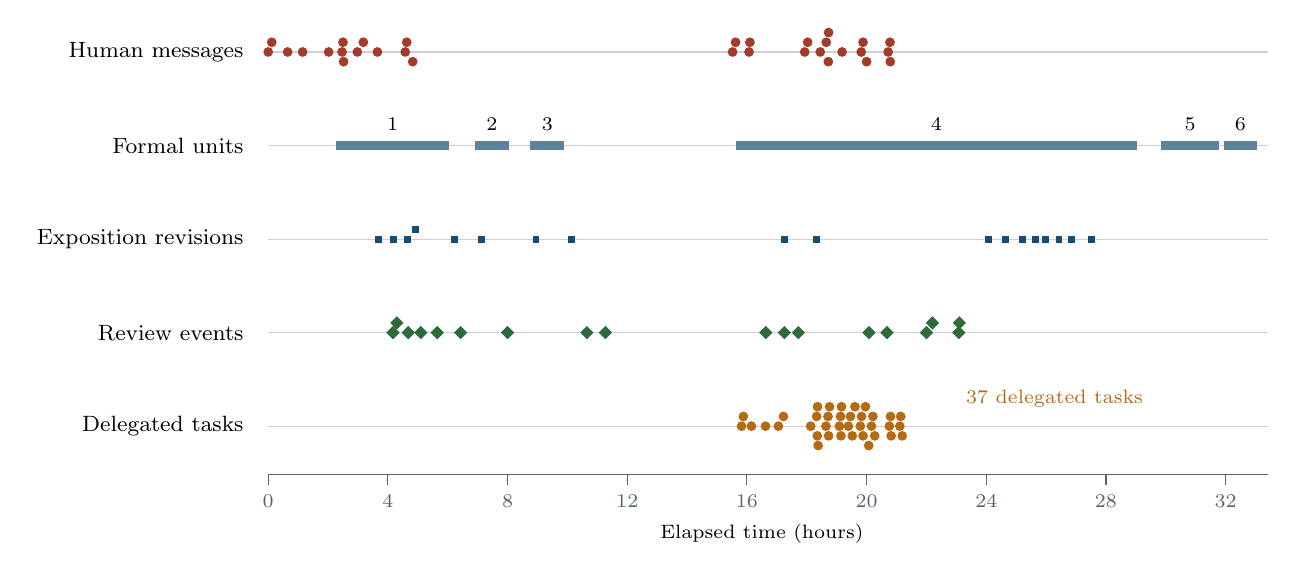
\begin{tikzpicture}[x=0.38cm,y=0.88cm,font=\footnotesize]
\node[anchor=east] at (-0.5,0) {Human messages};
\draw[planegray!30] (0,0)--(33.4,0);
\node[anchor=east] at (-0.5,-1.35) {Formal units};
\draw[planegray!30] (0,-1.35)--(33.4,-1.35);
\node[anchor=east] at (-0.5,-2.7) {Exposition revisions};
\draw[planegray!30] (0,-2.7)--(33.4,-2.7);
\node[anchor=east] at (-0.5,-4.05) {Review events};
\draw[planegray!30] (0,-4.05)--(33.4,-4.05);
\node[anchor=east] at (-0.5,-5.4) {Delegated tasks};
\draw[planegray!30] (0,-5.4)--(33.4,-5.4);
\node[circle,fill=humanred,inner sep=1.25pt] at (0,0.0) {};
\node[circle,fill=humanred,inner sep=1.25pt] at (0.12,0.14) {};
\node[circle,fill=humanred,inner sep=1.25pt] at (0.65,0.0) {};
\node[circle,fill=humanred,inner sep=1.25pt] at (1.15,0.0) {};
\node[circle,fill=humanred,inner sep=1.25pt] at (2.02,0.0) {};
\node[circle,fill=humanred,inner sep=1.25pt] at (2.47,0.0) {};
\node[circle,fill=humanred,inner sep=1.25pt] at (2.5,0.14) {};
\node[circle,fill=humanred,inner sep=1.25pt] at (2.52,-0.14) {};
\node[circle,fill=humanred,inner sep=1.25pt] at (2.98,0.0) {};
\node[circle,fill=humanred,inner sep=1.25pt] at (3.18,0.14) {};
\node[circle,fill=humanred,inner sep=1.25pt] at (3.65,0.0) {};
\node[circle,fill=humanred,inner sep=1.25pt] at (4.58,0.0) {};
\node[circle,fill=humanred,inner sep=1.25pt] at (4.63,0.14) {};
\node[circle,fill=humanred,inner sep=1.25pt] at (4.83,-0.14) {};
\node[circle,fill=humanred,inner sep=1.25pt] at (15.52,0.0) {};
\node[circle,fill=humanred,inner sep=1.25pt] at (15.62,0.14) {};
\node[circle,fill=humanred,inner sep=1.25pt] at (16.07,0.0) {};
\node[circle,fill=humanred,inner sep=1.25pt] at (16.1,0.14) {};
\node[circle,fill=humanred,inner sep=1.25pt] at (17.93,0.0) {};
\node[circle,fill=humanred,inner sep=1.25pt] at (18.03,0.14) {};
\node[circle,fill=humanred,inner sep=1.25pt] at (18.45,0.0) {};
\node[circle,fill=humanred,inner sep=1.25pt] at (18.65,0.14) {};
\node[circle,fill=humanred,inner sep=1.25pt] at (18.72,-0.14) {};
\node[circle,fill=humanred,inner sep=1.25pt] at (18.73,0.28) {};
\node[circle,fill=humanred,inner sep=1.25pt] at (19.18,0.0) {};
\node[circle,fill=humanred,inner sep=1.25pt] at (19.82,0.0) {};
\node[circle,fill=humanred,inner sep=1.25pt] at (19.88,0.14) {};
\node[circle,fill=humanred,inner sep=1.25pt] at (20.0,-0.14) {};
\node[circle,fill=humanred,inner sep=1.25pt] at (20.72,0.0) {};
\node[circle,fill=humanred,inner sep=1.25pt] at (20.78,0.14) {};
\node[circle,fill=humanred,inner sep=1.25pt] at (20.79,-0.14) {};
\node[rectangle,fill=linkblue,inner sep=1.25pt] at (3.7,-2.7) {};
\node[rectangle,fill=linkblue,inner sep=1.25pt] at (4.2,-2.7) {};
\node[rectangle,fill=linkblue,inner sep=1.25pt] at (4.66,-2.7) {};
\node[rectangle,fill=linkblue,inner sep=1.25pt] at (4.92,-2.56) {};
\node[rectangle,fill=linkblue,inner sep=1.25pt] at (6.23,-2.7) {};
\node[rectangle,fill=linkblue,inner sep=1.25pt] at (7.12,-2.7) {};
\node[rectangle,fill=linkblue,inner sep=1.25pt] at (8.95,-2.7) {};
\node[rectangle,fill=linkblue,inner sep=1.25pt] at (10.13,-2.7) {};
\node[rectangle,fill=linkblue,inner sep=1.25pt] at (17.25,-2.7) {};
\node[rectangle,fill=linkblue,inner sep=1.25pt] at (18.31,-2.7) {};
\node[rectangle,fill=linkblue,inner sep=1.25pt] at (24.08,-2.7) {};
\node[rectangle,fill=linkblue,inner sep=1.25pt] at (24.63,-2.7) {};
\node[rectangle,fill=linkblue,inner sep=1.25pt] at (25.2,-2.7) {};
\node[rectangle,fill=linkblue,inner sep=1.25pt] at (25.63,-2.7) {};
\node[rectangle,fill=linkblue,inner sep=1.25pt] at (25.98,-2.7) {};
\node[rectangle,fill=linkblue,inner sep=1.25pt] at (26.43,-2.7) {};
\node[rectangle,fill=linkblue,inner sep=1.25pt] at (26.85,-2.7) {};
\node[rectangle,fill=linkblue,inner sep=1.25pt] at (27.53,-2.7) {};
\node[diamond,fill=reviewgreen,inner sep=1.25pt] at (4.17,-4.05) {};
\node[diamond,fill=reviewgreen,inner sep=1.25pt] at (4.68,-4.05) {};
\node[diamond,fill=reviewgreen,inner sep=1.25pt] at (8.0,-4.05) {};
\node[diamond,fill=reviewgreen,inner sep=1.25pt] at (10.65,-4.05) {};
\node[diamond,fill=reviewgreen,inner sep=1.25pt] at (16.63,-4.05) {};
\node[diamond,fill=reviewgreen,inner sep=1.25pt] at (4.3,-3.9099999999999997) {};
\node[diamond,fill=reviewgreen,inner sep=1.25pt] at (5.1,-4.05) {};
\node[diamond,fill=reviewgreen,inner sep=1.25pt] at (5.65,-4.05) {};
\node[diamond,fill=reviewgreen,inner sep=1.25pt] at (6.43,-4.05) {};
\node[diamond,fill=reviewgreen,inner sep=1.25pt] at (17.25,-4.05) {};
\node[diamond,fill=reviewgreen,inner sep=1.25pt] at (11.27,-4.05) {};
\node[diamond,fill=reviewgreen,inner sep=1.25pt] at (17.72,-4.05) {};
\node[diamond,fill=reviewgreen,inner sep=1.25pt] at (20.08,-4.05) {};
\node[diamond,fill=reviewgreen,inner sep=1.25pt] at (20.68,-4.05) {};
\node[diamond,fill=reviewgreen,inner sep=1.25pt] at (22.0,-4.05) {};
\node[diamond,fill=reviewgreen,inner sep=1.25pt] at (22.2,-3.9099999999999997) {};
\node[diamond,fill=reviewgreen,inner sep=1.25pt] at (23.08,-4.05) {};
\node[diamond,fill=reviewgreen,inner sep=1.25pt] at (23.1,-3.9099999999999997) {};
\node[circle,fill=standorange,inner sep=1.25pt] at (15.82,-5.4) {};
\node[circle,fill=standorange,inner sep=1.25pt] at (15.88,-5.260000000000001) {};
\node[circle,fill=standorange,inner sep=1.25pt] at (16.15,-5.4) {};
\node[circle,fill=standorange,inner sep=1.25pt] at (16.62,-5.4) {};
\node[circle,fill=standorange,inner sep=1.25pt] at (17.05,-5.4) {};
\node[circle,fill=standorange,inner sep=1.25pt] at (17.22,-5.260000000000001) {};
\node[circle,fill=standorange,inner sep=1.25pt] at (18.13,-5.4) {};
\node[circle,fill=standorange,inner sep=1.25pt] at (18.33,-5.260000000000001) {};
\node[circle,fill=standorange,inner sep=1.25pt] at (18.35,-5.54) {};
\node[circle,fill=standorange,inner sep=1.25pt] at (18.36,-5.12) {};
\node[circle,fill=standorange,inner sep=1.25pt] at (18.38,-5.680000000000001) {};
\node[circle,fill=standorange,inner sep=1.25pt] at (18.64,-5.4) {};
\node[circle,fill=standorange,inner sep=1.25pt] at (18.71,-5.260000000000001) {};
\node[circle,fill=standorange,inner sep=1.25pt] at (18.73,-5.54) {};
\node[circle,fill=standorange,inner sep=1.25pt] at (18.76,-5.12) {};
\node[circle,fill=standorange,inner sep=1.25pt] at (19.09,-5.4) {};
\node[circle,fill=standorange,inner sep=1.25pt] at (19.13,-5.260000000000001) {};
\node[circle,fill=standorange,inner sep=1.25pt] at (19.14,-5.54) {};
\node[circle,fill=standorange,inner sep=1.25pt] at (19.16,-5.12) {};
\node[circle,fill=standorange,inner sep=1.25pt] at (19.39,-5.4) {};
\node[circle,fill=standorange,inner sep=1.25pt] at (19.46,-5.260000000000001) {};
\node[circle,fill=standorange,inner sep=1.25pt] at (19.52,-5.54) {};
\node[circle,fill=standorange,inner sep=1.25pt] at (19.61,-5.12) {};
\node[circle,fill=standorange,inner sep=1.25pt] at (19.79,-5.4) {};
\node[circle,fill=standorange,inner sep=1.25pt] at (19.83,-5.260000000000001) {};
\node[circle,fill=standorange,inner sep=1.25pt] at (19.88,-5.54) {};
\node[circle,fill=standorange,inner sep=1.25pt] at (19.96,-5.12) {};
\node[circle,fill=standorange,inner sep=1.25pt] at (20.07,-5.680000000000001) {};
\node[circle,fill=standorange,inner sep=1.25pt] at (20.16,-5.4) {};
\node[circle,fill=standorange,inner sep=1.25pt] at (20.21,-5.260000000000001) {};
\node[circle,fill=standorange,inner sep=1.25pt] at (20.27,-5.54) {};
\node[circle,fill=standorange,inner sep=1.25pt] at (20.76,-5.4) {};
\node[circle,fill=standorange,inner sep=1.25pt] at (20.8,-5.260000000000001) {};
\node[circle,fill=standorange,inner sep=1.25pt] at (20.82,-5.54) {};
\node[circle,fill=standorange,inner sep=1.25pt] at (21.11,-5.4) {};
\node[circle,fill=standorange,inner sep=1.25pt] at (21.14,-5.260000000000001) {};
\node[circle,fill=standorange,inner sep=1.25pt] at (21.19,-5.54) {};
\draw[line width=3pt,linkblue!70] (2.27,-1.35)--(6.04,-1.35);
\node[above,font=\scriptsize] at (4.155,-1.28) {1};
\draw[line width=3pt,linkblue!70] (6.9,-1.35)--(8.05,-1.35);
\node[above,font=\scriptsize] at (7.4750000000000005,-1.28) {2};
\draw[line width=3pt,linkblue!70] (8.76,-1.35)--(9.9,-1.35);
\node[above,font=\scriptsize] at (9.33,-1.28) {3};
\draw[line width=3pt,linkblue!70] (15.63,-1.35)--(29.03,-1.35);
\node[above,font=\scriptsize] at (22.330000000000002,-1.28) {4};
\draw[line width=3pt,linkblue!70] (29.85,-1.35)--(31.78,-1.35);
\node[above,font=\scriptsize] at (30.815,-1.28) {5};
\draw[line width=3pt,linkblue!70] (31.93,-1.35)--(33.05,-1.35);
\node[above,font=\scriptsize] at (32.489999999999995,-1.28) {6};
\draw[planegray] (0,-6.25)--(0,-6.1) node[below=4pt,font=\scriptsize] {0};
\draw[planegray] (4,-6.25)--(4,-6.1) node[below=4pt,font=\scriptsize] {4};
\draw[planegray] (8,-6.25)--(8,-6.1) node[below=4pt,font=\scriptsize] {8};
\draw[planegray] (12,-6.25)--(12,-6.1) node[below=4pt,font=\scriptsize] {12};
\draw[planegray] (16,-6.25)--(16,-6.1) node[below=4pt,font=\scriptsize] {16};
\draw[planegray] (20,-6.25)--(20,-6.1) node[below=4pt,font=\scriptsize] {20};
\draw[planegray] (24,-6.25)--(24,-6.1) node[below=4pt,font=\scriptsize] {24};
\draw[planegray] (28,-6.25)--(28,-6.1) node[below=4pt,font=\scriptsize] {28};
\draw[planegray] (32,-6.25)--(32,-6.1) node[below=4pt,font=\scriptsize] {32};
\draw[planegray] (0,-6.1)--(33.4,-6.1);
\node[font=\scriptsize] at (16.5,-6.95) {Elapsed time (hours)};
\node[anchor=west,font=\scriptsize,text=standorange] at (23,-5.0) {37 delegated tasks};
\end{tikzpicture}
\caption{Five execution lanes over the 33-hour AXIOM-$\Omega$ trace. Red circles mark 31 human messages in the first 22 hours. Six blue intervals run from formal-unit preregistration to merge; squares mark 18 accepted exposition revisions and diamonds mark recorded review events. The final lane contains 37 orange task markers (six early problem tasks and 31 derivation modules). Markers are displaced vertically to separate nearby recorded times; vertical position within a lane has no quantitative meaning. Formal-unit numbers 1--6 here enumerate the six accepted units, rather than the original task labels.}
\label{fig:timeline}
\end{figure}


Over those 33 hours, six kernel-verified Lean~4 units cleared all four
anti-inflation admission gates, five of them completing within 1~h~08~min to
3~h~46~min of public preregistration (three by hour 22, or roughly ten human
messages per accepted unit, and roughly five per unit across the full trace;
public issue and proof-contribution links appear in Table~\ref{tab:repro}).
Across 37 delegated cross-family tasks (six early problem tasks and 31
derivation modules, seven triggered by a coverage audit across 530 formal
statements in 226 expository units), two companion monographs grew within four
wall-clock hours from 52 and 48 pages to 270 and 192 pages (later reaching 284
and 195 pages), backed by 331 and 206 executable verification scripts and
2,352 example assertions. After two whole-paper adversarial review passes,
referees reported zero remaining false theorems in the reviewed drafts.

The loop also filtered out substantial flawed material before it could harden
into scientific slop. Fifty-two claims from source briefs, including
conjectures proposed by the team itself, were refuted and preserved with
explicit counterexamples, while 18 accepted bilingual exposition revisions (ten
initial contributions with an 18-minute median review cycle, plus eight
correction rounds carrying 87 refinements) kept the readable mathematics
aligned with the formal ledger. Table~\ref{tab:caught} details representative
catches across the separated review gates.

\begin{table}[htbp]
\centering\footnotesize
\caption{Representative mathematical defects and missed connections caught by
separated review gates in the 33-hour AXIOM-$\Omega$ trace.}
\label{tab:caught}
\begin{tabularx}{\linewidth}{@{}L{0.20\linewidth}L{0.19\linewidth}Y L{0.22\linewidth}@{}}
\toprule
Gate & Mechanism & Defect or opportunity caught & Resolution \\
\midrule
Library-first search & Frozen-ledger query & Dimension theorem already formally verified & Imported directly \\
Fresh-context referee & Cold snapshot review & Rigidity claim followed from Hurwitz; inputs misstated as outputs & Properly attributed; hypotheses restored \\
Cross-family adversarial review & Fresh Codex audit of delegated proof & Two subtle logical gaps in roundness theorem (compact spheres in dim 1, 3, 7) & Repaired and cross-verified by Claude author \& referee \\
Derivation status ledger & Delegated module checks & 52 source claims refuted, including team's own brief & Counterexamples and repaired statements kept \\
Author re-verification & Claude check of Codex bundle & Fabricated citation and probability error (0.145 versus 0.165) & Corrected before integration \\
Post-deposit formal review & Formal statement audit & One implication frozen without converse or necessity examples & Target amended; full equivalence frozen \\
Whole-paper re-review & Readable-proof audit & Five claims backed only by library pointers & Four proofs extracted; two prior settlements retrieved \\
\bottomrule
\end{tabularx}
\end{table}

The final catch demonstrates the value of insisting on readable exposition
instead of silent library pointers. When reviewers demanded self-contained
prose proofs, translating frozen Lean declarations back into readable
mathematics retrieved two open-conjecture settlements proved in the ledger six
weeks earlier: case~(ii) of the weighted B\"ottcher--Wenzel conjecture
(Mayumi--Kimura--Ohno--Chru\'sci\'nski, 2024) and width-three quantum
max-flow/min-cut for the bridge tensor network (Gesmundo--Lysikov--Steffan,
2025; pinned links in Table~\ref{tab:repro}). This step returned established
formal knowledge to human-digested exposition without double-counting either
result as a new formal settlement.

\section{Discussion, Future Outlook, Limitations and Conclusion}
\label{sec:discussion}
Scientific progress in the era of proof abundance depends directly on workflow
architecture. When autonomous agents operate without human framing or formal
grounding, novelty declines, overclaiming rises and prose referees overlook
fatal defects while generating costly false positives
\citep{societyai,oh2026slop,nguyen2026review,sun2026obligation}. Conversely,
when human researchers retain scientific direction and proof judgment while an
open, model-agnostic harness orchestrates derivation, counterexample search,
cold cross-family critique, executable review obligations and Lean~4 admission
gates, collaborative manuscripts outperform autonomous AI-only studies under
every tested frontier model family, match sound human preprints while
eliminating the unverified low-rigor tail, and bring living scholars directly
into checking proofs and repairing subtle gaps.

Human involvement remains foundational even as reasoning models advance. As
Terence Tao emphasizes in distinguishing proof generation from proof digestion
\citep{tao2026age}, a theorem enriches science only when living researchers
understand why it holds, pass the chalkboard test of explaining its conceptual
mechanism and see which frontier opens next. Across our live programme, 177
proof-checking scholars, 120 gap-repair collaborators, 1,995 pre-admission
formal-gate rejections and 52 early refutations inside a single 33-hour run
demonstrate how machine verification amplifies rather than replaces human
judgment: delegating routine checking and formal search frees scholars to focus
on taste, conceptual structure and scientific vision. Table~\ref{tab:principles}
distills eight transferable design principles from these mechanisms.

\begin{table}[htbp]
\centering\footnotesize
\caption{Eight transferable design principles for human-in-the-loop automated discovery.}
\label{tab:principles}
\begin{tabularx}{\linewidth}{@{}L{0.34\linewidth}Y@{}}
\toprule
Principle & Practical role in the research loop \\
\midrule
1. Keep humans in charge of direction & Retain human authority over questions (conjectures or intuitions), pivots and authorship. \\
2. Separate validity from substance & Pair kernel proofs with preregistration, library reuse and anti-inflation escape checks. \\
3. Store authoritative state externally & Keep objectives, snapshots, queues and gate records outside transient agent contexts. \\
4. Isolate authoring from critique & Review frozen snapshots cold across model families and recheck before integration. \\
5. Preserve refutations as evidence & Retain counterexamples, repairs and open obstacles so failed leads never recur. \\
6. Bind formal proofs to readable prose & Verify definition bridges and route manuscript disputes back to executable targets. \\
7. Enforce bounded execution & Scope credentials and sandboxes so agents never assume publication authority. \\
8. Close the loop with living scholars & Share readable proofs and formal links with experts to drive digestion and joint work. \\
\bottomrule
\end{tabularx}
\end{table}

\subsection{Future Outlook}
Four structural shifts emerge from pairing human scientific direction with
verification-centered automation. First, an open \emph{verification commons}
independent of any single model provider can convert proof abundance into
durable public infrastructure rather than opaque code dumps: interoperable
statement identities, pinned formal libraries and readable bilingual exposition
ensure that verified discoveries outlive any individual model family or
laboratory.

Second, \emph{executable peer review} offers a practical resolution to the
asymmetric review crisis identified by Sun et al.\ \citep{sun2026obligation}.
By requiring contested mathematical objections to compile into executable
Lean~4 targets, finite certificates or exact computational counterexamples,
peer review enforces an objective obligation threshold that filters out
ungrounded review slop and converts settled disputes into reusable library
theorems.

Third, recurring faculty reports of compressing months or an academic year of
solo exploratory derivation into a single week point toward a
``year-in-a-week'' collaborative rhythm across mathematics, quantum
information, mathematical physics, theoretical computer science, algorithm
design, economic theory and verified hardware or software. Within that rhythm,
scholars test bold intuitions rapidly, refute false leads within hours and
devote their creative energy to conceptual insight, proof checking and steering
the next frontier.

Fourth, verification-centered human-in-the-loop research reaches beyond
mathematics to any domain whose arguments rest on explicit definitions and
deductive consequence. Formal proof kernels do not adjudicate empirical
measurements or articles of faith, yet across formal philosophy, legal and
normative logic, and axiomatic traditions in theology and the philosophy of
religion, they can test exact logical entailment: clarifying which conclusions
genuinely follow from stated premises, exposing hidden assumptions and
constructing countermodels to flawed chains of reasoning. Extending the same
supervisory architecture into the empirical sciences replaces formal proof
kernels with executable experimental protocols, calibrated instrumentation and
independent laboratory replication, preserving the identical division between
human scientific judgment and non-circular verification.

\subsection{Limitations}
Several methodological and empirical boundaries govern how these results should
be interpreted. In the live programme, formal gates and workflow practices
evolved continuously without a randomized no-gate control arm; programme counts
of modules, dependency nodes and manuscripts index distinct objects rather than
additive discoveries, and an escape witness certifies non-trivial inference
relative to declared operations rather than scoring mathematical importance.
Scholar response rates and collaborative preprints likewise come from selected
observational outreach cohorts shaped by correspondence propensity and
unobserved abandoned lines, and faculty time-compression reports remain
qualitative.

In the 30-manuscript external benchmark, exact primary-category matching holds
between the two arXiv cohorts across six specialist classes, whereas the
ten-laboratory autonomous AI-only cohort comes from a keyword-ranked slice of a
separate empirical-ML agent society; differences in genre, citation style and
possible undisclosed AI assistance in contemporaneous human preprints can
therefore confound cross-cohort comparisons. Truncating texts at 36,000
characters omits proofs beyond that window, and although aggressive scrubbing
removed author headers, URLs and platform tags, retained titles, domain
terminology and occasional redaction markers prevent airtight
de-identification. While all three frontier judge families (OpenAI Codex
\code{gpt-6.1-sol}, Anthropic Claude \code{claude-opus-5-5} and Google Gemini),
every selection and blinding script and all 90 JSON evaluations are now
archived, shared pretraining distributions can still correlate model judgments,
and our exact permutation tests remain exploratory and unadjusted.

In the 20-claim mechanistic ablation, test propositions were extracted from
real theorems and counterexamples in our published arXiv corpus rather than an
external benchmark, and an executable verification-target gate can still miss a
genuine flaw when its generated verification script encounters a runtime or
symbolic-typing error (as occurred on one symbolic normalization test).
Longitudinal revision scores come from a separate nonrandomized paired study,
and case-study timings exclude prior infrastructure and unlogged human reading.
Prospective randomized studies should sample consecutive research lines, track
total human and compute cost, preregister component ablations and pair machine
checks with blinded specialist human referees.

\subsection{Conclusion}
Scientific discovery advances fastest when human researchers command direction
and understanding while automated systems shoulder derivation, refutation and
machine-checked verification. By uniting human scientific vision (from sharp
open conjectures to embryonic conceptual intuitions) and expert proof judgment
with an open model-agnostic harness, anti-inflation Lean~4 admission gates,
executable review obligations and direct collaboration with living scholars,
this methodology turns automated proof abundance into durable scientific
knowledge. Across 30 blinded public manuscripts scored by three independent
frontier model families, a 20-claim mechanistic ablation, a 24,925-PR public
admission-gate audit, 17 collaborative arXiv preprints and 177 proof-checking
scholars, these results establish a rigorous, transferable paradigm for
human-in-the-loop scientific discovery.

\clearpage
\appendix
\section{Programme Scope and Reproducibility Records}
\label{app:repro}
Table~\ref{tab:ops} defines the programme-wide scale measures cited in
Section~\ref{sec:production} at the 26 November 2026 snapshot (public PR gate
audit queried 27 November; case-study events occurred on 19--20 November); each
row measures a distinct research object and rows are not additive.
Table~\ref{tab:repro} lists public reproducibility sources, pinned revisions
and archived scripts; repository namespaces identify public code locations
rather than author affiliations.

\begin{table}[htbp]
\centering\footnotesize
\caption{Programme scope and measurement definitions at 26--27 November 2026.}
\label{tab:ops}
\begin{tabularx}{\linewidth}{@{}L{0.22\linewidth}L{0.34\linewidth}Y@{}}
\toprule
Research dimension & Measured scale & Measurement definition \\
\midrule
Formal knowledge base & 16,966 frozen Lean~4 modules; 24,810 Lean~4 source files & Frozen declaration collections and source files; neither counts independent theorems or discoveries \\[4pt]
Verified dependency graph & 18,367 nodes; 27,691 directed edges & Verified mathematical units and recorded dependency relations \\[4pt]
Resolved literature problems & 2,248 of 2,273 indexed problem records & Source-linked problems indexed as formally resolved; mathematical scope follows each source statement \\[4pt]
Public admission-gate audit & 24,925 completed PRs (22,930 merged; 1,995 closed unmerged); 5,447 escape registrations & All-time public gate throughput plus 1,000-PR recent window (Table~\ref{tab:ablation}B) and registered escape obligations \\[4pt]
Internal claim-review and formal-target pipeline & 212 drafts; 1,480 statements; 211 drafts linked to Lean~4 sources; 7 curated executable targets & Drafts, registered claims, source-linked drafts and selected formal propositions; linkage does not imply complete formalization \\[4pt]
External scholarly engagement & 485/1,049 replies (46.2\%); 316 positive assessments; 177 proof-checking participants; 120 gap-repair participants & Unique scholars; participation categories overlap; 223 collaborators span 230 threads, including 32 joint-paper threads; 70 opt-outs honoured \\[4pt]
Public collaborative preprints & 17 arXiv manuscripts; 16 with external coauthors (94.1\%) & Version-identified public outputs in Table~\ref{tab:corpus} \\[4pt]
External three-cohort benchmark & 30 manuscripts; 90 evaluations; overall 8.25 / 6.69 / 8.32 for collaboration & Ten manuscripts per cohort across three named model families ($W=0.828$; exact values in Table~\ref{tab:benchmark}) \\
\bottomrule
\end{tabularx}
\end{table}

\begingroup\footnotesize
\setlength{\LTpre}{4pt}\setlength{\LTpost}{4pt}
\begin{longtable}{@{}L{0.23\linewidth}L{0.72\linewidth}@{}}
\caption{Public scientific reproducibility records.}
\label{tab:repro}\\
\toprule Scientific source & Version and reproduction scope \\
\midrule\endfirsthead
\toprule Scientific source & Version and reproduction scope (continued) \\
\midrule\endhead
\midrule\multicolumn{2}{r}{\footnotesize Continued on next page}\\\endfoot
\bottomrule\endlastfoot
Formal verification repository &
\gh{the-omega-institute/trureturing/tree/99c5f79}{the-omega-institute/trureturing, revision 99c5f79}.
Frozen Lean~4 modules, problem records and formal admission registrations.
Escape-witness definitions are pinned at the
\gh{the-omega-institute/trureturing/tree/c382bd13}{c382bd13 source revision}.
Public PR gate audit queried on 27 November 2026 (\code{data/benchmark/exp3_trureturing_audit.json}).\\[5pt]
Six case-study formal units & Preregistration issues
\gh{the-omega-institute/trureturing/issues/31739}{31739},
\gh{the-omega-institute/trureturing/issues/31839}{31839},
\gh{the-omega-institute/trureturing/issues/31913}{31913},
\gh{the-omega-institute/trureturing/issues/32083}{32083},
\gh{the-omega-institute/trureturing/issues/32404}{32404},
\gh{the-omega-institute/trureturing/issues/32465}{32465}; corresponding merged proof contributions
\gh{the-omega-institute/trureturing/pull/31765}{31765},
\gh{the-omega-institute/trureturing/pull/31864}{31864},
\gh{the-omega-institute/trureturing/pull/31928}{31928},
\gh{the-omega-institute/trureturing/pull/32093}{32093},
\gh{the-omega-institute/trureturing/pull/32449}{32449},
\gh{the-omega-institute/trureturing/pull/32477}{32477}.
Proof-admission follow-up:
\gh{the-omega-institute/trureturing/pull/32533}{32533}.\\[5pt]
Earlier conjecture settlements & Weighted B\"ottcher--Wenzel case~(ii):
\gh{the-omega-institute/trureturing/issues/13715}{issue 13715},
\gh{the-omega-institute/trureturing/pull/14172}{proof contribution 14172}.
Bridge tensor network, width three:
\gh{the-omega-institute/trureturing/issues/14652}{issue 14652},
\gh{the-omega-institute/trureturing/pull/14787}{proof contribution 14787}.\\[5pt]
Autonomous external cohort ($n=10$) &
\href{https://huggingface.co/datasets/alphaXiv/AgentAlphaXiv}{alphaXiv/AgentAlphaXiv},
881 eligible studies. Top ten keyword-ranked studies from distinct laboratories:
\code{01a145e3-610} (Lab~2), \code{01a16e97-244} (Lab~5),
\code{01a097ed-5c1} (Lab~1), \code{01a174cd-9eb} (Lab~8),
\code{01a17a7e-3d3} (Lab~7), \code{01a18d0f-5a5} (Lab~12),
\code{01a18d5c-ae5} (Lab~13), \code{01a18ed0-e4f} (Lab~11),
\code{01a19561-135} (Lab~18), \code{01a1980a-8b3} (Lab~14).
All selection, blinding and scoring scripts are archived in \code{scripts/benchmark/}.\\[5pt]
Category-matched arXiv pairs ($n=10$) & Human-only / collaborative:
\code{quant-ph}: \arxiv{2610.21044v1} / \arxiv{2610.05623v2},
\arxiv{2611.00144v1} / \arxiv{2611.04568v1},
\arxiv{2611.00201v1} / \arxiv{2611.15431v1};
\code{math.CO}: \arxiv{2610.21036v1} / \arxiv{2610.24059v1},
\arxiv{2611.00126v1} / \arxiv{2611.03956v1},
\arxiv{2611.00145v1} / \arxiv{2611.21657v1};
\code{math.NT}: \arxiv{2610.21052v1} / \arxiv{2610.29608v1};
\code{cs.IT}: \arxiv{2610.21068v1} / \arxiv{2611.01064v1};
\code{math.GR}: \arxiv{2610.21600v2} / \arxiv{2610.20329v1};
\code{cs.FL}: \arxiv{2611.00153v1} / \arxiv{2610.39941v2}.\\[5pt]
Longitudinal arXiv records &
\arxiv{2610.05623v1}$\to$\arxiv{2610.05623v2} (30 days);
\arxiv{2609.09753v1}$\to$\arxiv{2609.09753v3} (41 days);
\arxiv{2609.25128v1}$\to$\arxiv{2609.25128v4} (20 days);
\arxiv{2610.18816v1}$\to$\arxiv{2610.18816v2} (2 days);
\arxiv{2610.39941v1}$\to$\arxiv{2610.39941v2} (12 days).
Table~\ref{tab:benchmark}C gives the separate version-blinded scores.\\[5pt]
Mechanistic ablation records &
Twenty blinded propositions (10 real flawed claims, 10 matched valid theorems from the collaborative arXiv corpus), prose verdicts (\code{claude-opus-5-5}, \code{gpt-6.1-sol}) and 20 executable Python verification scripts archived in \code{data/benchmark/ablation_obligation_threshold.json} and \code{scripts/benchmark/}.\\
\end{longtable}
\endgroup

\clearpage
\section{Collaborative arXiv Preprint Inventory}
\label{app:corpus}
Table~\ref{tab:corpus} lists all 17 preprints in ascending arXiv-ID order using
the primary identities reconciled on 26 November 2026 (normalizing one reversed
primary metadata record for Wenlin Zhang while retaining the raw record in the
manifest). Sixteen entries include external academic coauthors; reported scopes
summarize each linked preprint's stated results without claiming that every
external proof was rerun for this methodology study.
% Generated by scripts/render_corpus.py; edit the JSON manifest.
\begin{table}[htbp]\centering\small
\caption{Public output inventory, with exact arXiv versions.}\label{tab:corpus}
\begin{tabularx}{\linewidth}{@{}L{0.23\linewidth}Y@{}}
\toprule Version and field & Work and reported scope \\
\midrule
\arxiv{2607.04534v1}\par formal algebra and model evaluation & Mechanism-level routing failure in LLMs over Lean-verified algebraic structures\par\emph{Manuel Israel C\'{a}zares, Wenlin Zhang, Haobo Ma}\par\smallskip Proof-mechanism routing over Lean-verified algebraic objects \\[8pt]
\arxiv{2609.00706v1}\par automated reasoning & A Certificate-Producing Cascade for Equational Implication: The SAIR EQT2 Stage 2 Solver\par\emph{Haobo Ma, Wenlin Zhang, Manuel Israel C\'{a}zares}\par\smallskip Certificate-producing equational implication solver \\[8pt]
\arxiv{2609.09753v3}\par quantum information & Generalized Fidelity, the Data Processing Inequality, and Convexity\par\emph{Haobo Ma, Reza Rajaei, Wenlin Zhang}\par\smallskip Data-processing and convexity obstructions for generalized fidelity \\[8pt]
\arxiv{2609.25128v4}\par graph theory & Sub-quorum colorings of graphs\par\emph{Haobo Ma, Rafik Sahbi, Wenlin Zhang}\par\smallskip Structural bounds, algorithms and exact sub-quorum coloring values \\[8pt]
\arxiv{2609.33421v1}\par sequences and automata & A Padovan-automatic description of a nested recurrence\par\emph{Benoit Cloitre, Haobo Ma, Wenlin Zhang}\par\smallskip Finite-state description and exact properties of a nested recurrence \\[8pt]
\arxiv{2610.05623v2}\par quantum information & Approximation of a continuous-variable Gaussian state by discrete-variable quantum states\par\emph{Nicolae Cotfas, Haobo Ma, Wenlin Zhang}\par\smallskip Positivity and trace-norm-controlled discrete Gaussian approximation \\[8pt]
\arxiv{2610.18816v2}\par quantum information & On the coincidence of discrete and continuous definitions of Entanglement of Formation\par\emph{Haobo Ma, Maksim E. Shirokov, Wenlin Zhang}\par\smallskip Coincidence of discrete and continuous entanglement-of-formation definitions \\[8pt]
\arxiv{2610.20329v1}\par cellular automata & Generation by lazy and invertible cellular automata over the Klein four-group\par\emph{Edgar Alcal\'{a}-Arroyo, Alonso Castillo-Ramirez, Haobo Ma, Wenlin Zhang}\par\smallskip Characterization and cardinalities of a generated cellular-automaton submonoid \\[8pt]
\arxiv{2610.24059v1}\par graph theory & Sharp zero forcing numbers for the generalized Petersen graphs $P(n,3)$ and $P(n,4)$\par\emph{Arnav Krishnan, Haobo Ma, Wenlin Zhang}\par\smallskip Sharp zero forcing numbers for two generalized Petersen graph families \\[8pt]
\bottomrule\end{tabularx}\end{table}
\begin{table}[htbp]\ContinuedFloat\centering\small
\caption{Public output inventory, with exact arXiv versions (continued).}
\begin{tabularx}{\linewidth}{@{}L{0.23\linewidth}Y@{}}
\toprule Version and field & Work and reported scope \\
\midrule
\arxiv{2610.29608v1}\par number theory & Residue Sums Modulo Products of Two Distinct Odd Primes\par\emph{Haobo Ma, Mircea Merca, Wenlin Zhang}\par\smallskip Centered residue sums for cyclic subgroups modulo two odd primes \\[8pt]
\arxiv{2610.39941v2}\par combinatorics on words & Block-exchange descent for insertion: commuting projections and minimum masks\par\emph{Haobo Ma, Wenlin Zhang, Charles E. Hughes}\par\smallskip Block-exchange descent under commuting source projections; bounded computations \\[8pt]
\arxiv{2611.01064v1}\par information theory & Maximal input entropy for binary two-deletion and two-insertion channels\par\emph{Haobo Ma, Wenlin Zhang}\par\smallskip Exact entropy-maximizing binary words for two-deletion and two-insertion channels \\[8pt]
\arxiv{2611.03956v1}\par graph theory & Well-Covered Powers: Cartesian Products and Cayley Graphs\par\emph{Haobo Ma, Thanh Vu, Wenlin Zhang}\par\smallskip Well-covered graph powers, Cartesian products and Cayley classifications \\[8pt]
\arxiv{2611.04568v1}\par quantum information & Time-invariant negativity and persistent bound entanglement in a cyclic two-qutrit family\par\emph{Wenlin Zhang, Mazhar Ali, Haobo Ma}\par\smallskip Exact entanglement regions and dynamics for a cyclic two-qutrit family \\[8pt]
\arxiv{2611.15431v1}\par quantum information & Subadditivity and the failure of strong subadditivity in the Nichols--Wootters family of entropies\par\emph{Lin Zhang, Wenlin Zhang, Haobo Ma}\par\smallskip Proof of subadditivity (settling the subentropy conjecture) and failure of strong subadditivity across the Nichols--Wootters family \\[8pt]
\arxiv{2611.15815v1}\par sequences and recurrences & Meta-Nested Recurrences\par\emph{Beno\^{i}t Cloitre, Haobo Ma, Wenlin Zhang}\par\smallskip Golden-ratio bounds and Fibonacci orbit landings for variable-depth meta-nested recurrences; sharp error order for Grytczuk's fixed-depth recurrence \\[8pt]
\arxiv{2611.21657v1}\par enumerative combinatorics & Counting formulas and refined generating functions for inversion-sequence Classes 152 and 207\par\emph{Haobo Ma, Toufik Mansour, Wenlin Zhang}\par\smallskip Exact counting formula for Class 152 and Lambert-series generating functions for Class 207 inversion sequences \\[8pt]
\bottomrule\end{tabularx}
\end{table}


\clearpage
\section{Minimal Methodological Templates}
\label{app:templates}
These starter templates instantiate the shared-state and cross-family
delegation contracts of Sections~\ref{sec:methods} and~\ref{sec:architecture};
actual write permissions and external commitments remain governed by repository
policy and explicit human authorization.

\subsection*{C.1 Goal and State Record}
\begingroup\fontsize{8.5}{10}\selectfont
\begin{verbatim}
GOAL: <research direction or statement, source version and intended output>
AUTHORITY: <human decisions and applicable repository rules>
TARGET: <statement, hypotheses, boundary cases, admission basis>
REUSE: <library searches and exact existing results>
GATES: <written review, executable checks, kernel/CI scope>
BOUNDS: <measured resource limit and permitted concurrency>
STOP: <accepted artifact identity or precise remaining obstacle>
STATE (update after each material transition)
updated_utc: <time> | source_version: <immutable identifier>
phase: <derive | check | review | formalize | accepted | obstacle>
artifacts: <source identities and digests> | gate_results: <version, outcome>
next: <bounded action and responsible role>
\end{verbatim}
\endgroup

\subsection*{C.2 Cross-Family Delegation and Adversarial Review Protocol}
\begingroup\fontsize{8.5}{10}\selectfont
\begin{verbatim}
DELEGATION: Read <immutable snapshot>. Resolve <exact statement>.
Return a complete proof, explicit counterexample, or partial theorem
with the exact remaining gap. Preserve hypotheses and boundary cases.
Include primary citations, executable checks and claim evidence status.

FRESH REVIEW: Read the snapshot before the author's gap list.
For each central inference, give a justification, repairable gap,
or counterexample. Check definition changes, quantifiers, limits,
equality cases and the hypotheses of cited results.

INTEGRATION: Recheck the returned proof and scripts against the same
snapshot. Record the accepted digest and each unresolved dependency.
\end{verbatim}
\endgroup

\section*{Data and code availability}
Public artifact sources and pinned revisions appear in
Appendix~\ref{app:repro}, and exact collaborative arXiv versions in
Appendix~\ref{app:corpus}. Under \code{data/benchmark/}, the repository
archives all 90 named-model external benchmark JSON responses (OpenAI Codex,
Anthropic Claude and Google Gemini), the 30-manuscript manifest and summary,
the paired longitudinal revision records, the 20-claim mechanistic ablation
bundle and the 24,925-PR public gate audit (exact filenames in
Table~\ref{tab:repro}). All selection, blinding, scoring and permutation-test
scripts are archived under \code{scripts/benchmark/}, and
\code{scripts/render_benchmark.py} generates Table~\ref{tab:benchmark},
Figure~\ref{fig:benchmark} and Table~\ref{tab:ablation} directly from archived
JSON records. Correspondence findings are reported strictly as aggregate
scholar and thread counts, and starter workflow templates appear in
Appendix~\ref{app:templates}.

\section*{Statement on the use of AI}
In preparing this manuscript, the authors used AI tools (ChatGPT Pro, Codex, Claude and Gemini) for literature search, computation, checking and formal verification in Lean. All proofs can be checked by hand, and the computations can be reproduced from the accompanying verification package. The authors take full responsibility for the content.

\renewcommand{\bibfont}{\footnotesize\raggedright\interlinepenalty=10000}
\setlength{\bibsep}{0pt}
\bibliographystyle{plainnat}
\bibliography{references}
\end{document}
